% Document setup
\documentclass[12pt,a4paper,oneside]{article}
\usepackage[onehalfspacing]{setspace}
%\usepackage[utf8]{inputenc}	%Not needed when using XeLaTeX
%\usepackage[T1]{fontenc}
\usepackage{helvet}
\usepackage{fontspec}
\setmainfont{Free Helvetian}
\setlength\parindent{0cm}
\setlength\parskip{1em}
\usepackage{amsmath}
\usepackage{amssymb}
\usepackage{graphicx}
\usepackage{wrapfig}
\usepackage[toc,page]{appendix}
\usepackage{pdfpages}
\renewcommand{\appendixtocname}{Anhang}
\renewcommand{\appendixpagename}{Anhang}
\usepackage{natbib}	%citation
\usepackage{hyperref}	%clickable links
\usepackage{color}
\usepackage{listings}	%code listings
%%%%%%%%%%%%%%%%%%%%%%%%%%
\definecolor{lightgray}{rgb}{0.95, 0.95, 0.95}
\definecolor{darkgray}{rgb}{0.4, 0.4, 0.4}
%\definecolor{purple}{rgb}{0.65, 0.12, 0.82}
\definecolor{editorGray}{rgb}{0.95, 0.95, 0.95}
\definecolor{editorOcher}{rgb}{1, 0.5, 0} % #FF7F00 -> rgb(239, 169, 0)
\definecolor{editorGreen}{rgb}{0, 0.5, 0} % #007C00 -> rgb(0, 124, 0)
\definecolor{orange}{rgb}{1,0.45,0.13}		
\definecolor{olive}{rgb}{0.17,0.59,0.20}
\definecolor{brown}{rgb}{0.69,0.31,0.31}
\definecolor{purple}{rgb}{0.38,0.18,0.81}
\definecolor{lightblue}{rgb}{0.1,0.57,0.7}
\definecolor{lightred}{rgb}{1,0.4,0.5}
\lstdefinelanguage{CSS}{
	keywords={color,background-image:,margin,padding,font,weight,display,position,top,left,right,bottom,list,style,border,size,white,space,min,width, transition:, transform:, transition-property, transition-duration, transition-timing-function},	
	sensitive=true,
	morecomment=[l]{//},
	morecomment=[s]{/*}{*/},
	morestring=[b]',
	morestring=[b]",
	alsoletter={:},
	alsodigit={-}
}

% JavaScript
\lstdefinelanguage{JavaScript}{
	morekeywords={typeof, new, true, false, catch, function, return, null, catch, switch, var, if, in, while, do, else, case, break, let, of},
	morecomment=[s]{/*}{*/},
	morecomment=[l]//,
	morestring=[b]",
	morestring=[b]'
}

\lstdefinelanguage{HTML5}{
	language=html,
	sensitive=true,	
	alsoletter={<>=-},	
	morecomment=[s]{<!-}{-->},
	tag=[s],
	otherkeywords={>, <!DOCTYPE, <!doctype, </html, <html, <head, <title, </title, <style, </style, <link, </head, <meta, />, <li, </li, <ul, </ul, <h1, </h1, <h2, </h2, <img, <table, </table, <tr, </tr, <th, </th, <tr, </tr, <td, </td, <button, </button, <input, </input, <label, </label, </body, <body, </div, <div, </div>, </p, <p, </p>, </script, <script, <canvas, /canvas>, <svg, <rect, <animateTransform, </rect>, </svg>, <video, <source, <iframe, </iframe>, </video>, <image, </image>, <header, </header, <article, </article, <span, </span, <code, </code},
	ndkeywords={
		% General
		=,
		% HTML attributes
		charset=, src=, id=, width=, height=, style=, type=, rel=, href=,
		% SVG attributes
		fill=, attributeName=, begin=, dur=, from=, to=, poster=, controls=, x=, y=, repeatCount=, xlink:href=,
		% properties
		margin:, padding:, background-image:, border:, top:, left:, position:, width:, height:, margin-top:, margin-bottom:, font-size:, line-height:,
		% CSS3 properties
		transform:, -moz-transform:, -webkit-transform:,
		animation:, -webkit-animation:,
		transition:,  transition-duration:, transition-property:, transition-timing-function:,
	},
	deletekeywords={HTML, html}
}

\lstdefinestyle{htmlcssjs} {%
	% General design
	%  backgroundcolor=\color{editorGray},
	basicstyle={\footnotesize\ttfamily},   
	frame=b,
	% line-numbers
	xleftmargin={0.75cm},
	numbers=left,
	stepnumber=1,
	firstnumber=1,
	numberfirstline=true,	
	% Code design
	identifierstyle=\color{black},
	keywordstyle=\color{blue}\bfseries,
	ndkeywordstyle=\color{editorGreen}\bfseries,
	stringstyle=\color{editorOcher}\ttfamily,
	commentstyle=\color{brown}\ttfamily,
	% Code
	language=HTML5,
	alsolanguage=JavaScript,
	alsodigit={.:;},	
	tabsize=2,
	showtabs=false,
	showspaces=false,
	showstringspaces=false,
	extendedchars=true,
	breaklines=true,
	% German umlauts
	literate=%
	{Ö}{{\"O}}1
	{Ä}{{\"A}}1
	{Ü}{{\"U}}1
	{ß}{{\ss}}1
	{ü}{{\"u}}1
	{ä}{{\"a}}1
	{ö}{{\"o}}1
}

%%%%%%%%%%%%%%%%%%%%%%%%%%%%%%%%%


\hypersetup{	%link formatting
	colorlinks=true,
	linkcolor=blue,
	filecolor=magenta,      
	urlcolor=cyan,
	citecolor=green,
	linktoc=page,
	pdftitle={\@title},
	pdfpagemode=FullScreen,
}
\def\sectionautorefname{Abschnitt}
\def\subsectionautorefname{Abschnitt}
\def\subsubsectionautorefname{Abschnitt}
\def\tableautorefname{Tabelle}
\def\figureautorefname{Abbildung}
\def\appendixautorefname{Anhang}
\usepackage{enumitem}
\setlist[itemize]{noitemsep, topsep=0pt}
\usepackage[left=3cm, right=3cm, top=3cm, bottom=3cm]{geometry}
\usepackage[ngerman]{babel}
\author{Lorenz Bung}
\title{Analyse der didaktischen Auswirkungen von Klassenteilungen auf die Unterrichtsplanung bei einer Jahrgangsstufe 2 des Technischen Gymnasiums mit Profilfach Technik und Management}
\date{\today}

\begin{document}
	\newgeometry{left=3cm, top=5cm, right=3cm, bottom=5cm}
\makeatletter
\begin{titlepage}
	\Large
	\centering
	\@title
	\vfill
	\Huge
	\textbf{Dokumentation des Forschungsprojekts in angewandter Fachdidaktik Informatik}
	\vfill
	\normalsize
	\begin{tabular*}{\linewidth}{@{\extracolsep{\fill}} ll}
		Vorgelegt von: & \@author \\
		Datum: & \@date \\
		Semester / Matr.-Nr.: & SS24 / 5113060 \\
		Betreuende Lehrkraft: & OStR Benjamin Lempp \\
		Ausbildungsschule: & RFGS Freiburg
	\end{tabular*}
\end{titlepage}
\makeatother
\restoregeometry
	\newpage
	\thispagestyle{empty}
	\vspace*{0cm}
\begin{center}
\Large
\textbf{Versicherung}\\
\vspace{1.5cm}
\end{center}
\normalsize
Hiermit versichere ich, dass ich diese Dokumentation des Forschungsprojekts selbstständig und nur mit den angegebenen Hilfsmitteln angefertigt habe.
Ich habe für alle Stellen und Materialien, die dem Wortlaut oder dem Sinn nach aus anderen Werken (auch aus elektronischen Medien) entnommen wurden, die Quellen angegeben.\\
\vspace{3cm}\\
\rule{0.3\textwidth}{0.4pt} \hspace{0.1\textwidth} \rule{0.6\textwidth}{0.4pt}\\
(Ort, Datum) \hspace{0.24\textwidth} (eigenhändige Unterschrift)
	\newpage
	\tableofcontents
	\thispagestyle{empty}
	\pagenumbering{gobble}
	\newpage
	\setcounter{page}{1}
	\pagenumbering{arabic}
	\section{Einleitung}
	\section{Konzeption}
\label{sec:konzeption}

\subsection{Voraussetzungsanalyse}
\label{subsec:voraussetzungsanalyse}

Die in dieser Arbeit durchgeführte Voraussetzungsanalyse orientiert sich am von Paul Heimann begründeten Berliner Modell \cite[S.~41--70]{arnold2015}.
\begin{figure}[h!]
	\centering
	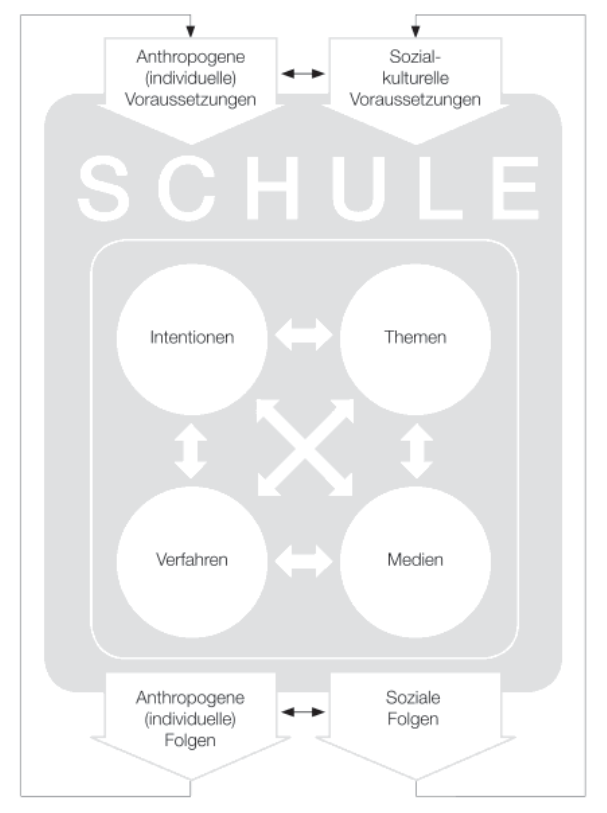
\includegraphics[width=0.6\textwidth]{media/BerlinerModell.png}
	\caption{Schematische Darstellung des Berliner Modells \cite[S.~68]{arnold2015}}
	\label{fig:berliner-modell}
\end{figure}
Wie in \autoref{fig:berliner-modell} zu sehen ist, spielen nach diesem Modell sowohl die anthropogenen als auch die sozio-kulturellen Voraussetzungen der Lerngruppe eine entscheidende Rolle.
Im Folgenden wird daher auf diese beiden Bedingungen genauer eingegangen, mögliche Auswirkungen auf die Lerngruppe genannt und daraus resultierende Konsequenzen auf die Planung des Unterrichts diskutiert.\\\\

\subsubsection{Anthropogene Voraussetzungen}
\label{subsubsec:anthropogene-voraussetzungen}

Bei der Analyse der anthropogenen Voraussetzungen der Lerngruppe werden Faktoren berücksichtigt, welche die Schülerinnen und Schüler in die Unterrichtssituation mitbringen.
Fragen, die diese Analyse zu beantworten sucht, können unter Anderem die folgenden sein:
\begin{itemize}
	\item Welches Vorwissen bringt die Lerngruppe zum Thema der Unterrichtsstunde mit?
	\item Wie sind die sozialen Vorbedingungen, die innerhalb der Klasse herrschen?
	\item Wie sind Selbstwahrnehmung und Interesse der Schülerinnen und Schüler in Bezug auf das Fach, insbesondere zum aktuellen Thema?
\end{itemize}

Die im Rahmen dieser Arbeit durchgeführte Unterrichtseinheit fand in der zweiten Jahrgangsstufe eines Technischen Gymnasiums mit dem Profilfach ``Technik und Management'' statt.
Viele der Schülerinnen und Schüler haben zuvor eine Realschule besucht und dort die Mittlere Reife erhalten.
Das technische Gymnasium bietet ihnen somit die Möglichkeit, statt einer Ausbildung einen höheren Bildungsabschluss zu erlangen.
Für viele der Schülerinnen und Schüler ist die Perspektive nach dem Abitur ein Studium.
Unter Anderem aus diesem Grund brachten die meisten Lernenden eine vergleichsweise hohe Eigenmotivation mit.

Die Wahl der Schule und des Profilfaches spricht dafür, dass der Großteil der Lerngruppe ein hohes Interesse an technisch-mathematischen Themenbereichen mitbringt.
In Hospitationen im Unterricht mit der Klasse hat sich durch Gespräche und Beobachtungen jedoch herauskristallisiert, dass Informatik und informatische Inhalte von Teilen der Klasse als langweilig oder irrelevant empfunden wird.
Andere Schülerinnen und Schüler brachten bereits Einiges an Vorwissen mit und hatten auch Spaß an der Auseinandersetzung mit Problemstellungen aus dem Informatikunterricht.

Der Grund für die Wahl des Themas dieser Forschungsarbeit war, dass die Klasse für den Unterricht in zwei etwa gleich große Gruppen geteilt wurde.
Das Klassenklima in der Klasse lässt sich als durchgängig gut beschreiben, allerdings ist hierbei zu berücksichtigen, dass die Sicht der Lehrkraft auf das Klassenklima selbstverständlich nicht immer exakt der realen Situation entspricht.
Auffällig an vielen Klassen am Technischen Gymnasium -- insbesondere aber auch bei der in dieser Arbeit betrachteten Lerngruppe -- ist das ungleiche Geschlechterverhältnis.
In diesem konkreten Fall waren im Unterricht nur zwei Schülerinnen, während der Rest der Lerngruppe männlich war.
Aufgrund möglicher geschlechtsspezifischer Stereotypen, die insbesondere im Fach Informatik leider immer noch sehr prävalent sind, ist dieses ungleiche Geschlechterverhältnis ein Punkt, auf den bei der Durchführung des Unterrichts und der eventuell angepassten Konzeption der darauffolgenden Stunde ein besonderes Augenmerk gelegt werden muss.

Ein großes Problem vor der Durchführung der Unterrichtseinheit war die fehlende Klarheit über das Vorwissen der Schülerinnen und Schüler zum Thema ``Webentwicklung''.
Auch die betreuende Lehrkraft konnte diesbezüglich keine Angaben machen, da diese die Klasse erst in der Jahrgangsstufe übernommen hatte, nicht jedoch in der Eingangsklasse.
Eben dann steht allerdings das Thema ``HTML und CSS'' im Bildungsplan \cite[BPE~2]{bildungsplan-tg-informatik}, was essentielles Vorwissen für die kommende Unterrichtseinheit ist.
Diese Frage konnte bis zur ersten Stunde auch nicht mehr geklärt werden, was die Planung dieser ersten Stunde erheblich erschwerte.
Klar war aber, dass alle Schülerinnen und Schüler Erfahrung im Bereich der Programmierung mit Python mitbrachten.
Dies war das Thema, mit dem sich die Klasse bis dahin beschäftigt hatte; es lag also auch noch keine große zeitliche Distanz dazwischen.

Insgesamt kann festgehalten werden, dass die Lerngruppe in Bezug auf ihr Vorwissen zwar relativ homogen war, bezüglich der Motivation für das Fach und seine Lerninhalte jedoch große Heterogenität herrschte.
Dies spiegelte sich auch deutlich in der Lerngeschwindigkeit der verschiedenen Schülerinnen und Schüler wider und war bei der weiteren Planung der Unterrichtseinheit zu berücksichtigen.

\subsubsection{Sozio-kulturelle Voraussetzungen}
\label{subsubsec:sozio-kulturelle-voraussetzungen}

Hinter der Frage nach den sozio-kulturellen Voraussetzungen stehen sowohl externe wie auch innere Faktoren, die das Unterrichtsgeschehen beeinflussen können. Ein Teil der dazu zählenden Punkte sind:
\begin{itemize}
	\item Wie viel Zeit steht für den Unterricht zur Verfügung?
	\item Handelt es sich um eine Einzel- oder eine Doppelstunde?
	\item In welchen Räumlichkeiten findet die Stunde statt?
	\item Genügt die vorhandene technische Ausstattung den Anforderungen des geplanten Unterrichts?
\end{itemize}
Die Räumlichkeiten der Richard-Fehrenbach-Gewerbeschule, in der der im Rahmen dieser Arbeit durchgeführte Unterricht stattgefunden hat, sind durchgängig als technisch gut bis sogar hervorragend ausgestattet einzustufen.
Sämtliche gehaltenen Stunden konnten in Computerräumen von ausreichender Größe durchgeführt werden, so dass jede Person an einem eigenen Computer arbeiten konnte.
Zudem war in jedem Raum eine digitale Tafel mit Dokumentenkamera und drahtloser Verbindung zu digitalen Endgeräten vorhanden.
Weiterhin war in jedem Computerraum ein Drucker platziert, so dass bei Bedarf Übungs- und Merkblätter in gedruckter Form an die Schülerinnen und Schüler weitergegeben werden konnten.

Alle Stunden der Unterrichtseinheit waren Doppelstunden, also in ununterbrochener Länge von 90 Minuten.
Geplant waren für das gesamte Thema 8 Stunden bzw. 4 Doppelstunden, was sich mit den Vorgaben im Bildungsplan deckt \cite[BPE~19]{bildungsplan-tg-informatik}.
Bei Bedarf wäre es allerdings möglich gewesen, dies um eine weitere Doppelstunde zu erweitern.
Insgesamt wurden 32 Stunden \'a 45 Minuten gehalten, wobei jede Stunde einmal pro Gruppe stattgefunden hat.
Je Gruppe fanden also 16 Stunden \'a 45 Minuten, jeweils in Blöcken von 90 Minuten statt.


\subsection{Lerninhalte und -ziele}
\label{subsec:lernziele}

Vor der Aufstellung konkreter Lernziele ist es notwendig, sich klar zu machen, welche Lerninhalte im Unterricht eigentlich vermittelt werden sollen.
Für die Planung einer vollständigen Bildungsplaneinheit, wie es in der vorliegenden Arbeit stattgefunden hat, muss dafür zunächst eine Aufteilung der Lernstoffes in einzelne Abschnitte durchgeführt werden, welche dann wiederum die inhaltliche Grundlage für die einzelnen Stunden bieten.
Es ist also nötig, das Thema der Einheit in möglichst unabhängig voneinander stehende Abschnitte zu gliedern, welche aber gleichzeitig im Gesamtbild miteinander in Wechselwirkung stehen und ein umfassendes Bild der Thematik liefern.

Dass diese Trennung eine große Herausforderung darstellt, ist wohl selbstverständlich.
Viel bedeutsamer ist für diese Arbeit jedoch, dass es nicht die eine unanfechtbar korrekte Lösung für dieses Problem gibt, sondern dass viele verschiedene Aufteilungen des Lernstoffes möglich sind.
Je nach Lerngruppe, Vorwissen oder insbesondere auch nach verfolgtem Ziel haben diese verschiedenen Herangehensweisen unterschiedliche Vor- und Nachteile, über die man sich bei der Planung des Unterrichts im Klaren sein muss.


\subsubsection{Gliederung des Lernstoffs}
\label{subsubsec:lernstoff-gliederung}

Bei der Planung der in dieser Arbeit betrachteten Bildungsplaneinheit zum Thema ``Javascript'' gab es dabei zunächst zwei Ansätze, den Lernstoff zu gliedern.
Der erste Ansatz war, analog zu bereits erfolgten Stunden zum Thema ``Python'' vorzugehen und Javascript einfach von Grund auf als neue Programmiersprache einzuführen.
Dieser Ansatz hatte den Vorteil, dass das Vorgehen bereits in der Unterrichtseinheit zu Python erfolgreich durchgeführt worden war und man mit dieser Methode ein relativ sicheres Lernergebnis erreichen können würde.
Der große Nachteil war jedoch, dass eine erneute Einführung einer neuen Programmiersprache nach demselben Schema und mit ähnlichen oder sogar gleichen Übungsaufgaben für die Schülerinnen und Schüler sehr langweilig gewesen wäre.
Hier hätte sich schnell die Sinnfrage gestellt: ``Wir haben das doch schon alles in Python gemacht, warum sollen wir das erneut in Javascript machen?''
Sicherlich wäre diese Frage zumindest teilweise gerechtfertigt gewesen; außerdem wäre der Kernunterschied von Javascript zu Python nicht klar geworden:
Nämlich, dass es sich bei Javascript um eine im Browser clientseitig ausgeführte Sprache handelt.

Im Gegensatz dazu stand der zweite Ansatz, der darauf aufbaute, direkt von Anfang an zu zeigen, dass das Ziel der Einheit die Webentwicklung ist.
Hier würden Aufgaben so gestellt werden, dass die Schülerinnen und Schüler bereits vorgefertigte Webseiten inklusive Codegerüsten bekommen würden und diese entsprechend den Aufgabenstellungen vervollständigen müssten.
Die Einführung bekannter Programmierkonzepte wie Verzweigungen, Schleifen und Funktionen würde nicht als abstraktes Konzept, sondern direkt anhand von Beispielen eingeführt werden.
Ein entscheidender Vorteil wäre hierbei, dass sich die erlernten Konzepte direkt auf reale in der Webentwicklung auftretende Situationen anwenden ließe und sich so direkt erschließen würde, wofür das ganze benötigt wird.
Dies würde im Optimalfall zu erhöhter Motivation bei den Schülerinnen und Schülern führen.
Der entscheidende Nachteil dieser Variante wäre jedoch, dass die Struktur des Unterrichts weniger klar wäre.
Da sich die Einführung neuer Konzepte an Beispielproblemen wie vorgefertigten Webseiten orientieren würde, müssten viele Teile des Codes bereits fertig vorliegen.
Dies könnte die Schülerinnen und Schüler ablenken und im schlechtesten Fall so verwirren, dass die eigentlich einfachen Aufgaben nicht mehr gelöst werden könnten.
Andererseits böte sich hier auch die Chance, interessierten Schülerinnen und Schülern einen Ausblick auf fortgeschrittenere Inhalte zu bieten.


\subsubsection{Formulierung der Lernziele}
\label{subsubsec:formulierung-lernziele}

Die in \autoref{subsubsec:lernstoff-gliederung} diskutierten Ansätze wurden mit der betreuenden Lehrkraft ausgiebig besprochen und die Vor- und Nachteile gegeneinander abgewägt.
Schlussendlich wurde für die Planung der Unterrichtseinheit der zweite, problemorientierte Ansatz gewählt.
Einer der  ausschlaggebenden Gründe dafür war der motivationsaufbauende Aspekt von problemorientiertem Unterricht, insbesondere vor dem Hintergrund, dass die Programmiersprache Python erst kürzlich formal eingeführt worden war.
Weiterhin bot die natürliche Komplexität der Aufgaben eine gute Möglichkeit, bereits erste Maßnahmen zur Differenzierung zu nehmen und durch zusätzliche bzw. weiterführende Inhalte auch besonders schnellen oder interessierten Schülerinnen und Schülern gerecht zu werden.

Ein Teil der im Bildungsplan zum Thema Javascript verankerten Lerninhalte \cite[BPE~19]{bildungsplan-tg-informatik} sind die folgenden:

\begin{itemize}
	\item Deklaration von Variablen und Konstanten
	\item Einfache arithmetische Vergleichsoperationen
	\item Kontrollstrukturen: Verzweigungen, Schleifen
\end{itemize}

Eine Aufteilung dieser Inhalte auf die vier Doppelstunden lieferte die in \autoref{tab:stundenplanung-vorher} dargestellte Struktur.
Wie sich im Verlauf der verschiedenen Stunden zeigen sollte, war diese Planung nicht final und musste im Laufe der Zeit noch weiteren Änderungen unterzogen werden.
Weiteres hierzu wird in \autoref{TODO} \textcolor{red}{TODO} genauer diskutiert.

\begin{table}[h!]
	\begin{tabular*}{\linewidth}{l|l}
		\hline
		\textbf{Stunde} & \textbf{Inhalt}\\
		\hline
		1 & Überprüfung des Vorwissens zu HTML/CSS\\
		& Variablen\\
		& if-Verzweigung\\
		\hline
		2 & Schleifen: for/while\\
		\hline
		3 & Arrays, Funktionen\\
		\hline
		4 & Entwicklung eines kleinen Spiels auf Basis der erlernten Konzepte\\
		\hline
	\end{tabular*}
	\caption{Aufteilung der Lerninhalte auf die Unterrichtsstunden vor der Durchführung}
	\label{tab:stundenplanung-vorher}
\end{table}

Aufgrund der Vorerfahrungen der Schülerinnen und Schüler bei der Programmierung mit Python konnte davon ausgegangen werden, dass die grundlegenden Konzepte der Programmierung wie Variablen, Schleifen und Verzweigungen nicht erneut auf theoretisch-abstraktem Niveau besprochen werden mussten.
Aus diesem Grund und auch der geringen syntaktischen Unterschiede war nur eine Doppelstunde für die Themen Variablen und if-Verzweigungen geplant.
Die auf diesen Überlegungen basierenden Lernziele sind in \autoref{tab:lernziele-1-vorher} genauer beschrieben.

\begin{table}[h!]
\begin{tabular*}{\linewidth}{l|l}
	\hline
	\textbf{Zielart} & \textbf{Lernziel}\\
	\hline \hline
	Grobziel & Die Schülerinnen und Schüler beschreiben die Struktur von HTML-\\
	& und CSS-Dokumenten.\\
	Feinziel & Die SuS nennen Beispiele für HTML-Tags.\\
	Feinziel & Die SuS beurteilen die Korrektheit von CSS-Dokumenten bezüglich\\
	& ihrer Syntax.\\
	Grobziel & Die SuS identifizieren Unterschiede und Gemeinsamkeiten der\\
	& Syntax von Variablen und Verzweigungen in Javascript und Python.\\
	Feinziel & Die SuS identifizieren Code als Python- oder Javascript-Code.\\
	Feinziel & Die SuS nennen Unterschiede in der Syntax von if-Verzweigungen\\
	& in Javascript und Python.\\
	Feinziel & Die SuS beurteilen die Qualität von Javascript-Code hinsichtlich\\
	& seiner syntaktischen Korrektheit.\\
	\hline
\end{tabular*}
\caption{Planung der Lernziele für die erste Doppelstunde vor ihrer Durchführung}
\label{tab:lernziele-1-vorher}
\end{table}

Ebenso sollten for- und while-Schleifen beide in einer Doppelstunde besprochen werden.
Beide Strukturen waren bereits aus der Unterrichtseinheit zu Python bekannt und mussten daher nicht erst neu eingeführt werden.
In \autoref{tab:lernziele-2-vorher} sind die dazu formulierten Lernziele zu finden.

\begin{table}[h!]
\begin{tabular*}{\linewidth}{l|l}
	\hline
	\textbf{Zielart} & \textbf{Lernziel}\\
	\hline \hline
	Grobziel & Die SuS verwenden for- und while-Schleifen, um Code wiederholt\\
	& ausführen zu lassen.\\
	Feinziel & Die SuS differenzieren zwischen korrekter und inkorrekter Syntax\\
	& bei for- und while-Schleifen in Javascript.\\
	Feinziel & Die SuS nennen Unterschiede und Gemeinsamkeiten von for- und\\
	& while-Schleifen in Javascript und in Python.\\
	Feinziel & Die SuS formulieren for-Schleifen in while-Schleifen um und\\
	& umgekehrt.\\
	Feinziel & Die SuS argumentieren, ob für ein gegebenes Problem eher eine\\
	& for- oder eine while-Schleife geeignet ist.\\
	\hline
\end{tabular*}
\caption{Planung der Lernziele für die zweite Doppelstunde vor ihrer Durchführung}
\label{tab:lernziele-2-vorher}
\end{table}

Die für die dritte Stunde vorgesehenen Inhalte Arrays bzw. Listen und Funktionen waren so geplant, dass schnellere Schülerinnen und Schüler direkt in dieser Doppelstunde damit fertig werden würden, allerdings auch bei Bedarf die Möglichkeit bestand, noch die darauffolgende vierte Doppelstunde dafür zu nutzen.
Die in \autoref{tab:lernziele-3-vorher} dargestellten Lernziele sind daher nur in Bezug auf die schnelleren Schülerinnen und Schüler gültig; sie können auch erst in der vierten Doppelstunde erfüllt werden.

\begin{table}[h!]
\begin{tabular*}{\linewidth}{l|l}
	\hline
	\textbf{Zielart} & \textbf{Lernziel}\\
	\hline \hline
	Grobziel & Die SuS implementieren die aus Python bekannte Struktur der Liste\\
	& in der neuen Programmiersprache Javascript.\\
	Feinziel & Die SuS nutzen die Methode \texttt{indexOf()}, um den Index eines\\
	& Elements in einer Liste zu bestimmen.\\
	Feinziel & Die SuS nutzen Indizes, um auf bestimmte Elemente in einer Liste\\
	& zuzugreifen.\\
	Feinziel & Die SuS identifizieren Unterschiede und Gemeinsamkeiten der\\
	& Syntax von Listen bei Javascript und Python.\\
	Grobziel & Die SuS verwenden Funktionen, um ihren Code zu strukturieren.\\
	Feinziel & Die SuS unterscheiden korrekte von inkorrekter Syntax bezüglich\\
	& vorgegebenen Codes zu Funktionen in Javascript.\\
	Feinziel & Die SuS unterscheiden zwischen Funktionsaufruf und -rumpf.\\
	Feinziel & Die SuS rufen vorgegebene Funktionen korrekt auf.\\
	Feinziel & Die SuS implementieren Funktionen anhand eines vorgegebenen\\
	& Funktionskopfes und Beschreibung der Funktionalität.\\
	\hline
\end{tabular*}
\caption{Planung der Lernziele für die dritte Doppelstunde vor ihrer Durchführung}
\label{tab:lernziele-3-vorher}
\end{table}

\begin{table}[h!]
	\begin{tabular*}{\linewidth}{l|l}
		\hline
		\textbf{Zielart} & \textbf{Lernziel}\\
		\hline \hline
		Grobziel & Die SuS implementieren die Logik eines browserbasierten Spiels\\
		& mithilfe von Javascript.\\
		Feinziel & Die SuS analysieren Problemstellungen in Bezug auf deren\\
		& Umsetzung durch Programmierkonzepte.\\
		Feinziel & Die SuS identifizieren algorithmische Lösungen für komplexe\\
		& Programmierproblemstellungen.\\
		Feinziel & Die SuS nutzen Schleifen, Listen, Verzweigungen und Funktionen,\\
		& um ihren Code sinnvoll zu strukturieren.\\
		Grobziel & Die SuS kombinieren erlernte Programmiertechniken und wenden\\
		& diese im Zusammenspiel miteinander an.\\
		\hline
	\end{tabular*}
	\caption{Optionale und zusätzliche Lernziele für die vierte Doppelstunde vor ihrer Durchführung}
	\label{tab:lernziele-4-vorher}
\end{table}

Leistungsstarke Lernende würden die Zeit der vierten Doppelstunde dann nutzen können, um ihr in der Einheit gelerntes Wissen anzuwenden und ein kleines browserbasiertes Spiel wie Tic-Tac-Toe zu entwickeln.
Für diese Schülerinnen und Schüler ergäben sich somit zusätzliche, über die reine Programmiertechnik hinausgehende Lernziele, welche in \autoref{tab:lernziele-4-vorher} aufgelistet sind.
Das Erreichen dieser Lernziele ist somit nicht für alle Schülerinnen und Schüler verpflichtend, sondern eine freiwillige Zusatzleistung, welche der Festigung und Vertiefung des Stoffes dient.


\subsection{Methodik und Medien}
\label{subsec:methodik-medien}

Unter Anderem aufgrund der guten technischen Ausstattung der Schule war eine vielfältige Gestaltung des Unterrichts möglich.
Nach Rücksprache mit der betreuenden Lehrkraft erfolgte die Einführung in neue Inhalte, beispielsweise die Syntax einer if-Verzweigung in der ersten Stunde, durch direkte Instruktion.
Dies basierte auf früheren Erfahrungen mit der Klasse, welche nahelegten, dass diese Methode zu vergleichsweise wenigen Ablenkungen seitens der Schülerinnen und Schüler führte.
Gleichzeitig wurde so ein schneller Einstieg in die neue Thematik geschaffen und damit ein zügiger Übergang in das selbstständige und schülerzentrierte Arbeiten.

Für die Arbeitsphasen wurde den Schülerinnen und Schülern folgendes Material zur Verfügung gestellt:
\begin{itemize}
	\item Merkblätter, auf denen die in der Erarbeitungsphase kennengelernten Inhalte in kompakter und verständlicher Form erneut aufbereitet waren und somit als Arbeitshilfe genutzt werden konnten.
	Die Merkblätter finden sich in \autoref{app:merkblätter}.
	\item Arbeitsblätter, auf welchen sich die Aufgabenstellungen für die aktuelle Doppelstunde finden ließen.
	Diese sind in \autoref{app:übungsblätter} einsehbar.
	\item Zu den Aufgaben gehörige Codegerüste, welche neben dem von den Schülerinnen und Schülern zu bearbeitendem Javascript-Code auch auf HTML und CSS basierende Webseiten enthielten, um die praxisorientierten Aufgaben direkt testen zu können.
	Screenshots des Codes finden sich in \autoref{app:codegerüste}.
\end{itemize}
Sämtliches Material lag grundsätzlich in digitaler Form vor und wurde über das Tauschlaufwerk der Schule kommuniziert.
Zusätzlich bot sich den Schülerinnen und Schülern die Möglichkeit, auf Nachfrage Merk- und Arbeitsblätter auszudrucken, um diese in analoger Form als zusätzliche Hilfe bei der Arbeit vor sich liegen zu haben.

Weiterhin wurde bereits zu Beginn der Unterrichtseinheit kommuniziert, dass zur Information oder auch zur Weiterbildung für Interessierte zahlreiche Onlineressourcen zur Verfügung stehen.
Insbesondere wurde die weit verbreitete Webseite \href{https://www.w3schools.com}{w3schools} genannt, welche neben Tutorials zu HTML, CSS, Javascript und weiteren Programmiersprachen auch Referenzdokumente zu oben genannten Komponenten der Webentwicklung zur Verfügung stellt \cite{w3schools}.

Zusätzlich wurden auch Online-Quizzes verwendet, allgemeiner bekannt unter dem Namen ``Kahoot''.
Neben den positiven Erfahrungen, die Lehrkräfte bei ihren Klassen mit dem Format sammeln konnten \cite{dellos2015kahoot}, kann der Ansatz des game-based learning mithilfe von Kahoot positive Effekte auf Lernerfolge, Motivation und Ängste der Schülerinnen und Schüler haben sowie das Klassenklima verbessern \cite{wang2020kahoot}.
Eingesetzt wurde das Tool sowohl bei Unterrichtseinstiegen zur Vorwissensaktivierung und Motivationsaufbau, als auch innerhalb von Übungsphasen zur Sammlung des Gruppenfokus.
	\section{Umsetzung}
	\section{Reflexion}
	\bibliographystyle{plain}
\bibliography{bibliography}
	\pagenumbering{Roman}
\begin{appendices}
\section{Unterrichtsverlaufspläne}
\label{app:unterrichtsverlaufspläne}

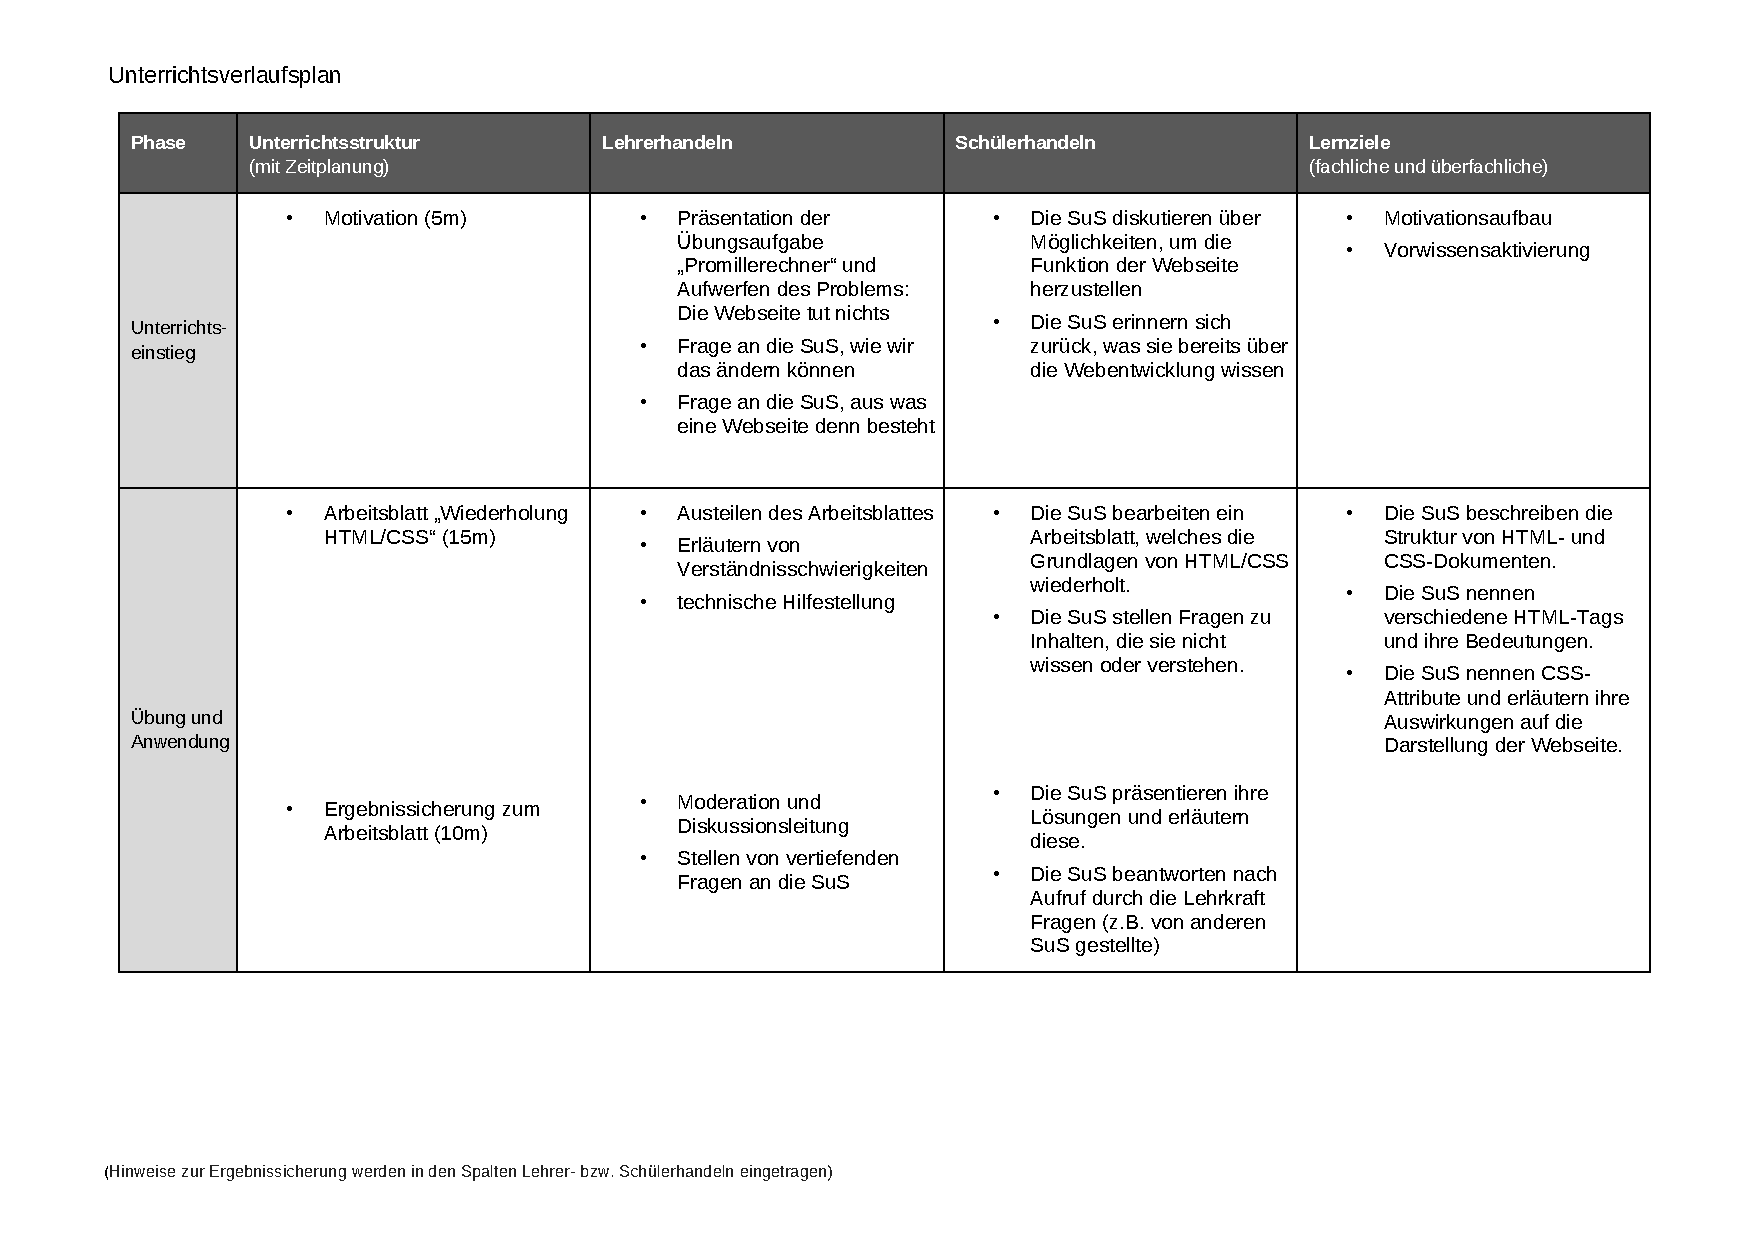
\includepdf[pages={-}, angle=90, scale=0.8, frame, pagecommand={\thispagestyle{plain}},
addtotoc={1, subsection, 2, Unterrichtsverlaufsplan 1, subsec:UVP1}]{appendix/Javascript1/Unterrichtsverlaufsplan.pdf}
\label{pdf:UVP1}
\pagebreak

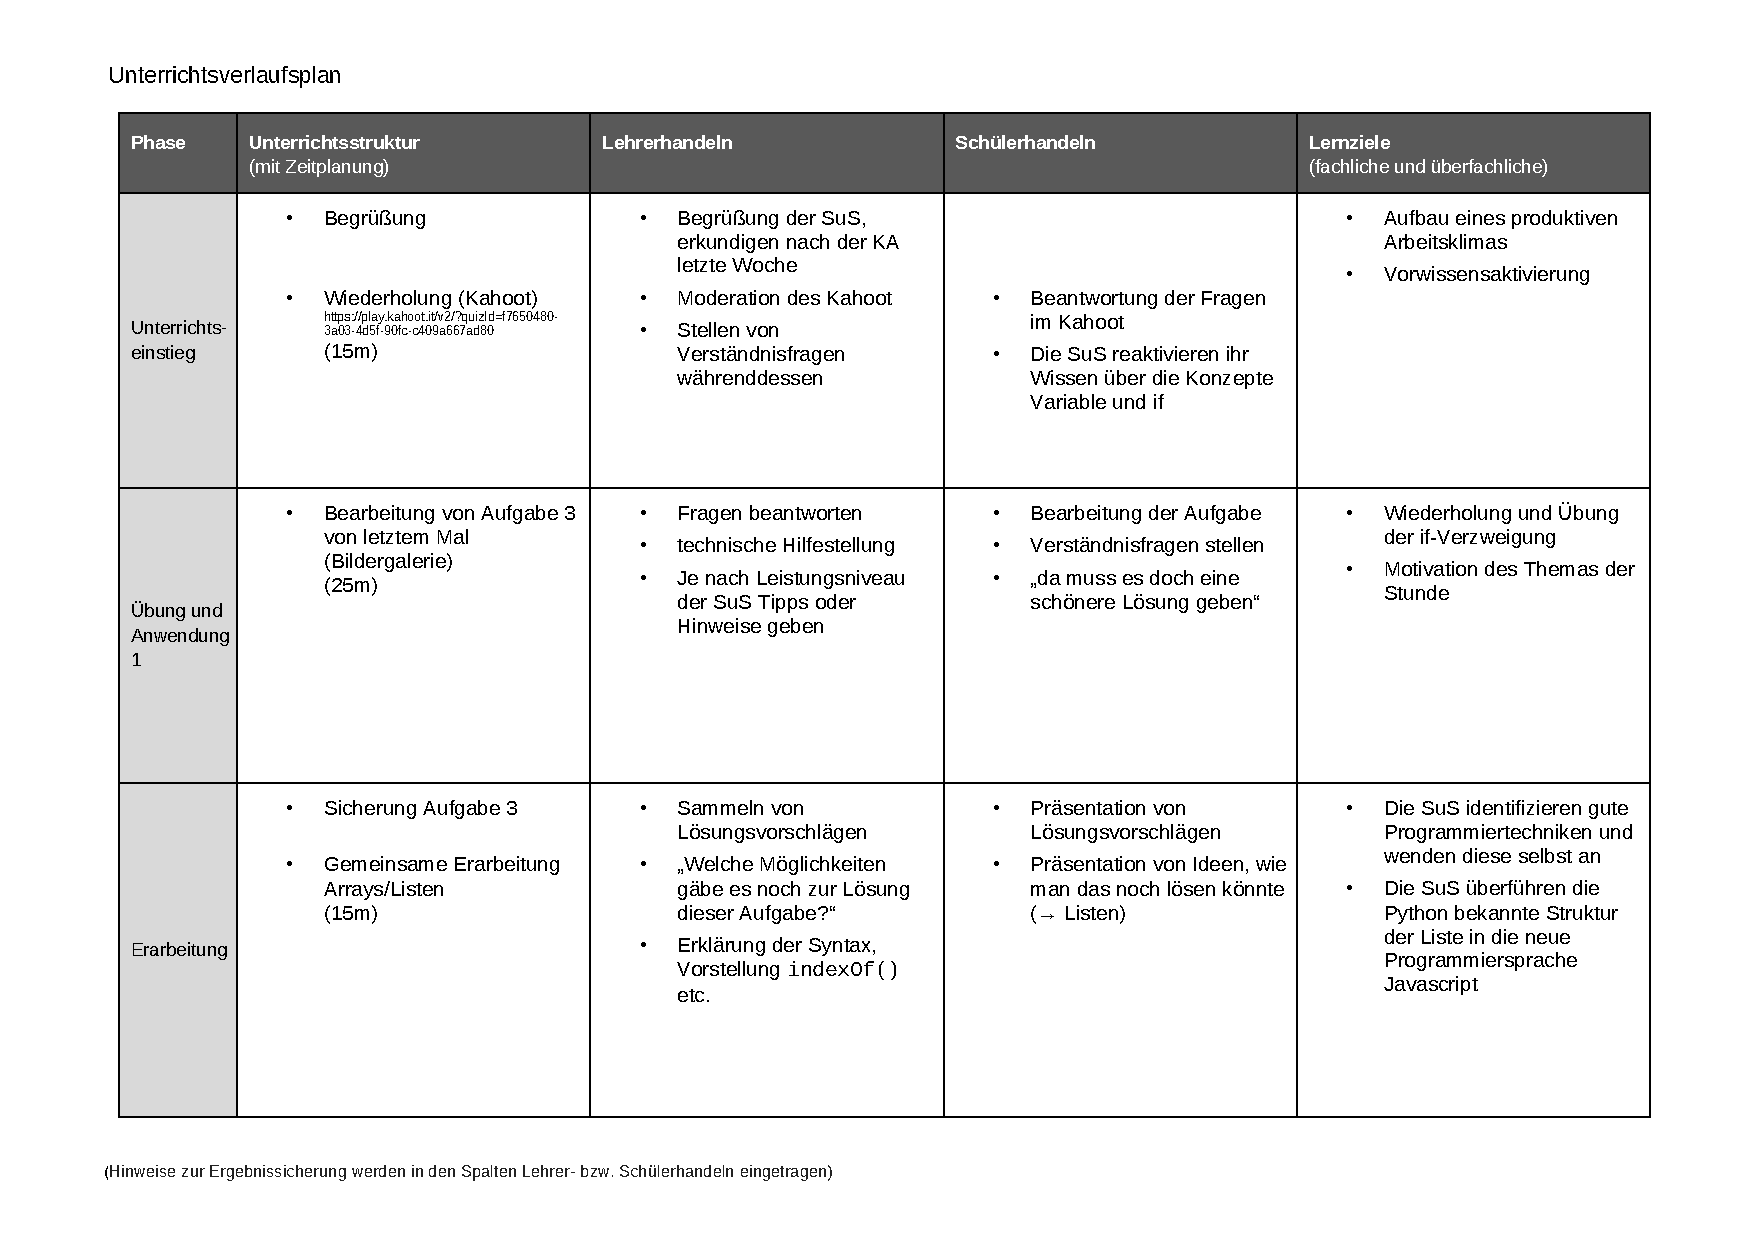
\includepdf[pages={-}, angle=90, scale=0.8, frame, pagecommand={\thispagestyle{plain}},
addtotoc={1, subsection, 2, Unterrichtsverlaufsplan 2, subsec:UVP2}]{appendix/Javascript2/Unterrichtsverlaufsplan.pdf}
\label{pdf:UVP2}
\pagebreak

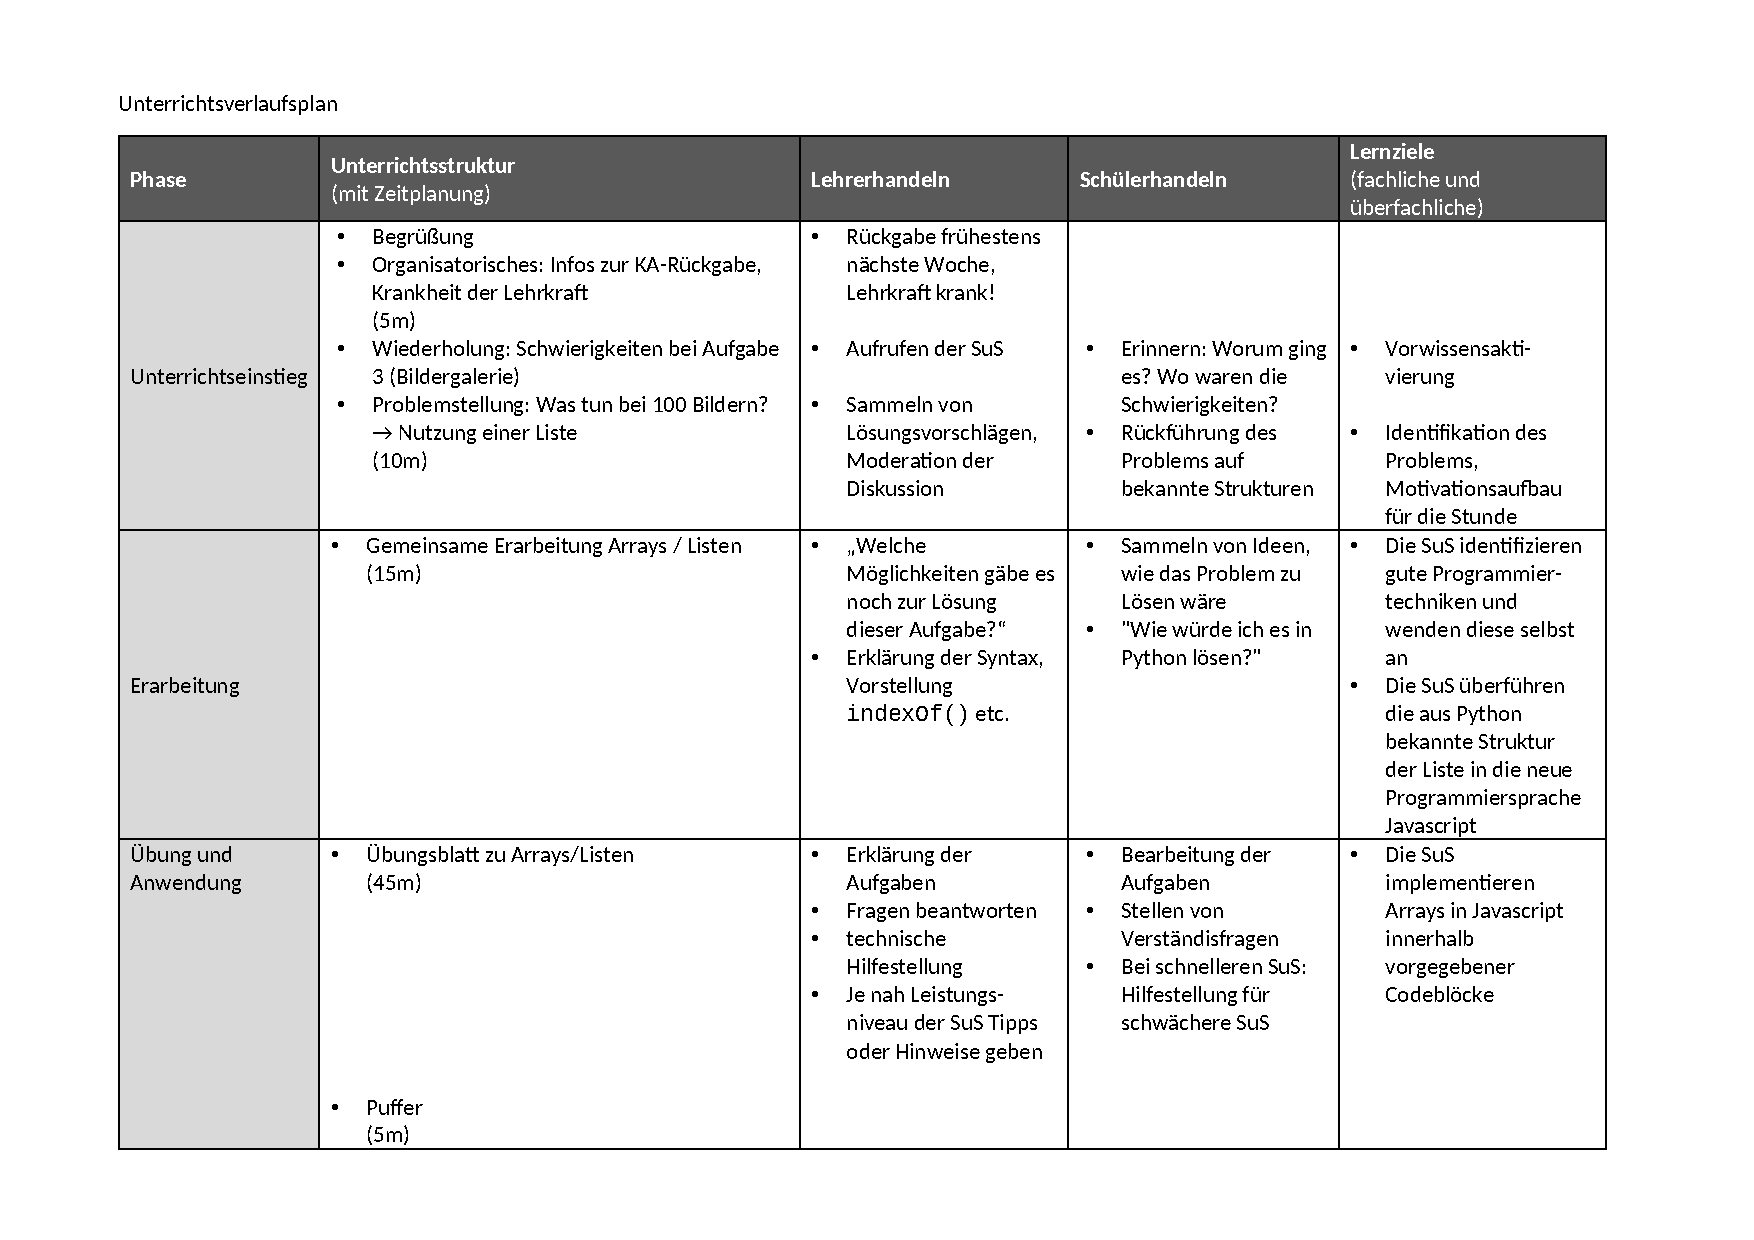
\includepdf[pages={-}, angle=90, scale=0.8, frame,
pagecommand={\thispagestyle{plain}},
addtotoc={1, subsection, 2, Unterrichtsverlaufsplan 3, subsec:UVP3}]{appendix/Javascript3/Unterrichtsverlaufsplan.pdf}
\label{pdf:UVP3}
\pagebreak

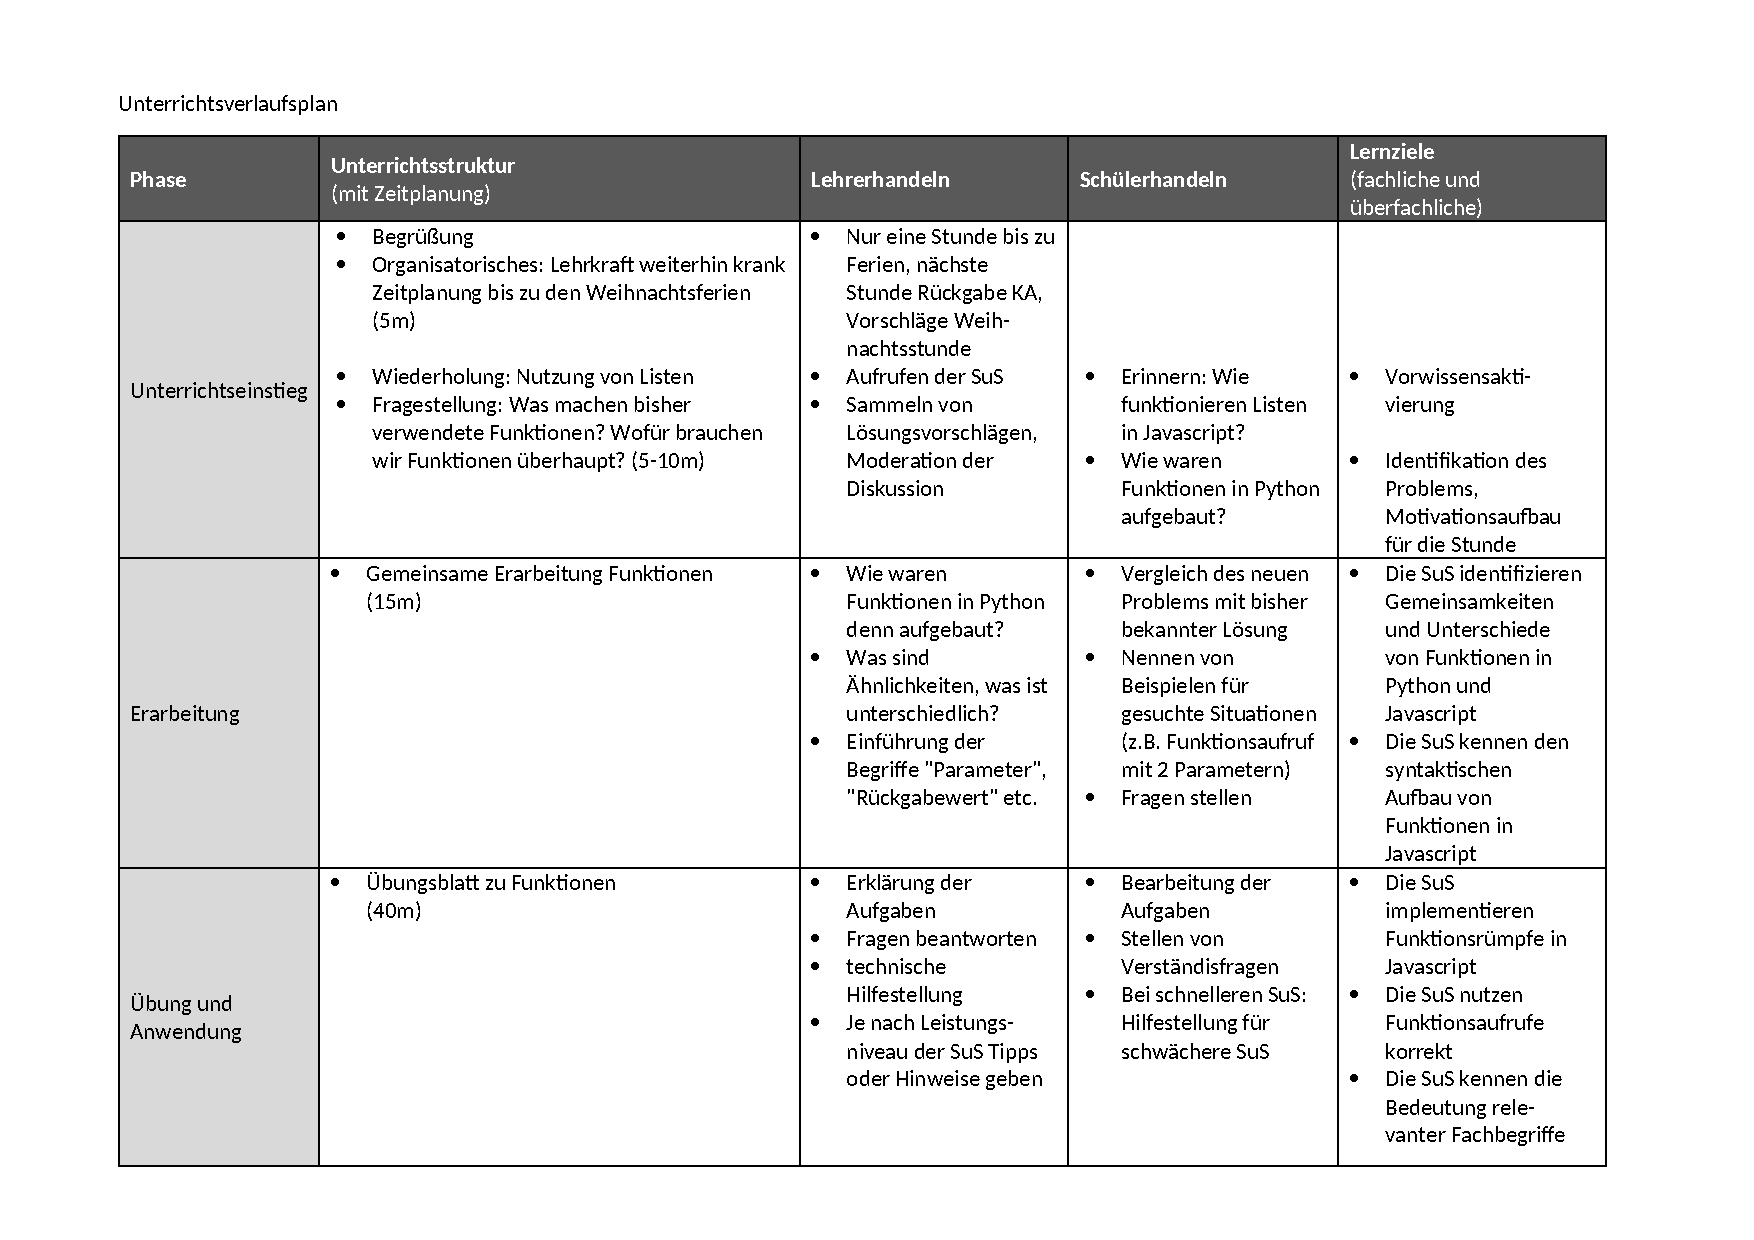
\includepdf[pages={-}, angle=90, scale=0.8, frame,
pagecommand={\thispagestyle{plain}},
addtotoc={1, subsection, 2, Unterrichtsverlaufsplan 4, subsec:UVP4}]{appendix/Javascript4/Unterrichtsverlaufsplan.pdf}
\label{pdf:UVP4}
\pagebreak


\section{Merkblätter}
\label{app:merkblätter}
\pagebreak

\phantomsection
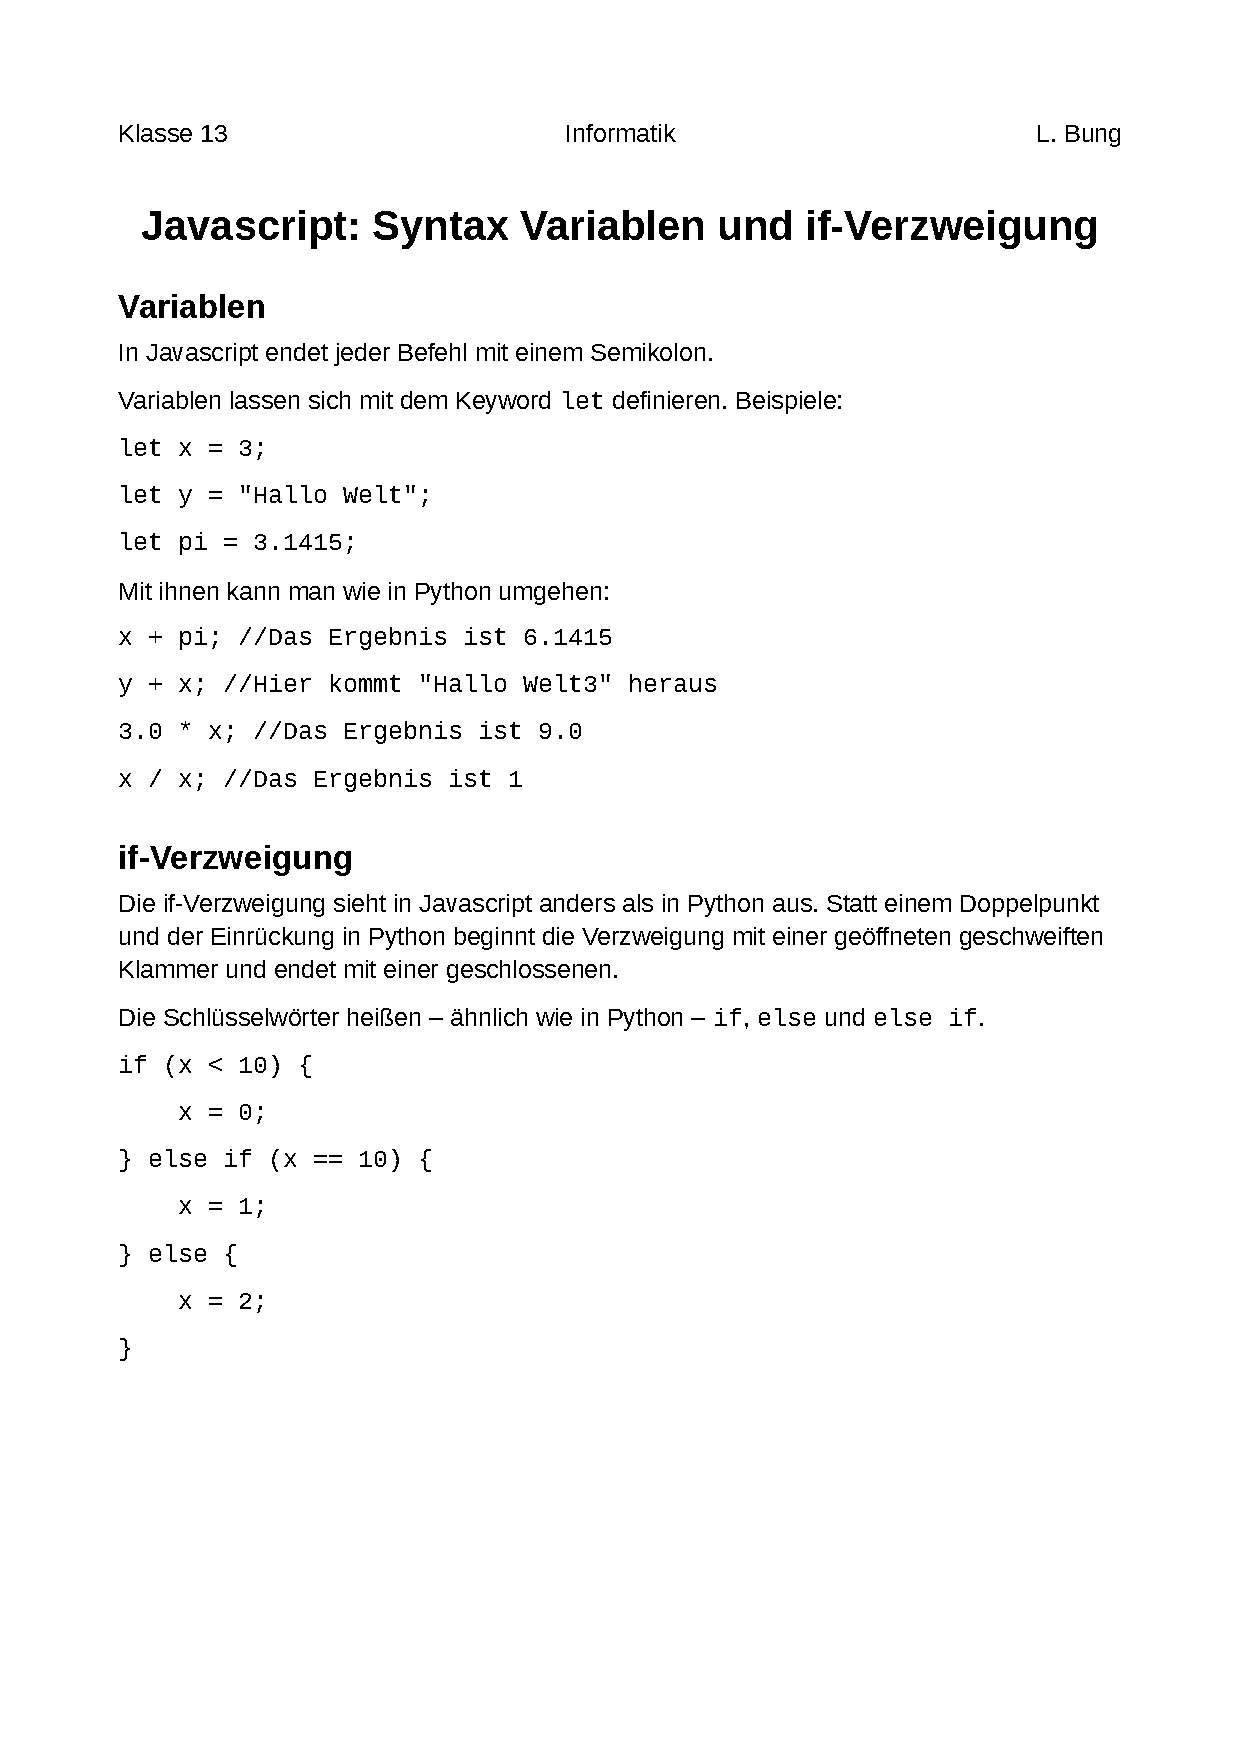
\includepdf[pages={-}, scale=0.8, frame, pagecommand={\thispagestyle{plain}},
addtotoc={1, subsection, 2, Merkblatt Variablen/if, subsec:merkblatt_variablen_if}]{appendix/Javascript1/Merkblatt_Variablen_if.pdf}
\label{pdf:merkblatt_variablen_if}
\pagebreak

\phantomsection
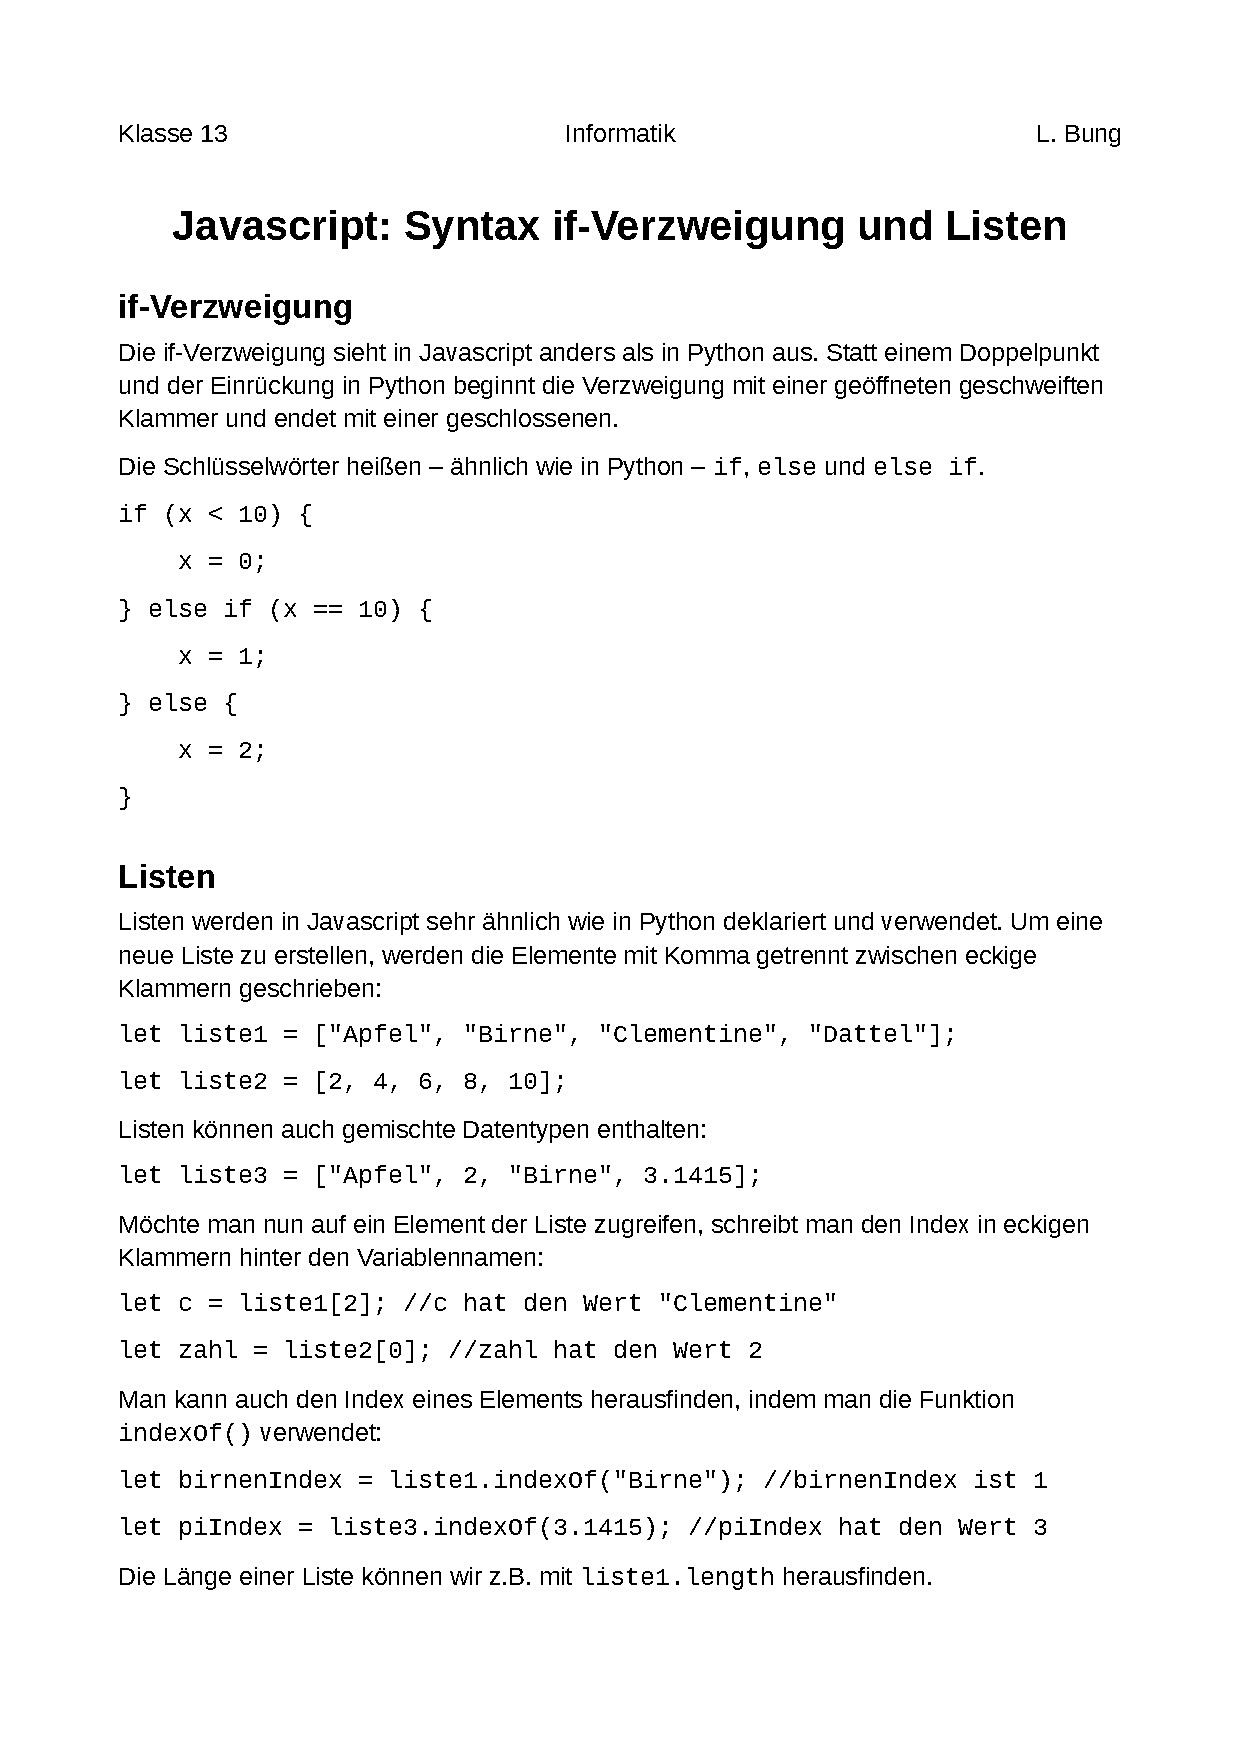
\includepdf[pages={-}, scale=0.8, frame, pagecommand={\thispagestyle{plain}},
addtotoc={1, subsection, 2, Merkblatt if/Listen, subsec:merkblatt_if_listen}]{appendix/Javascript3/Merkblatt_if_Listen.pdf}
\label{pdf:merkblatt_if_listen}
\pagebreak

\phantomsection
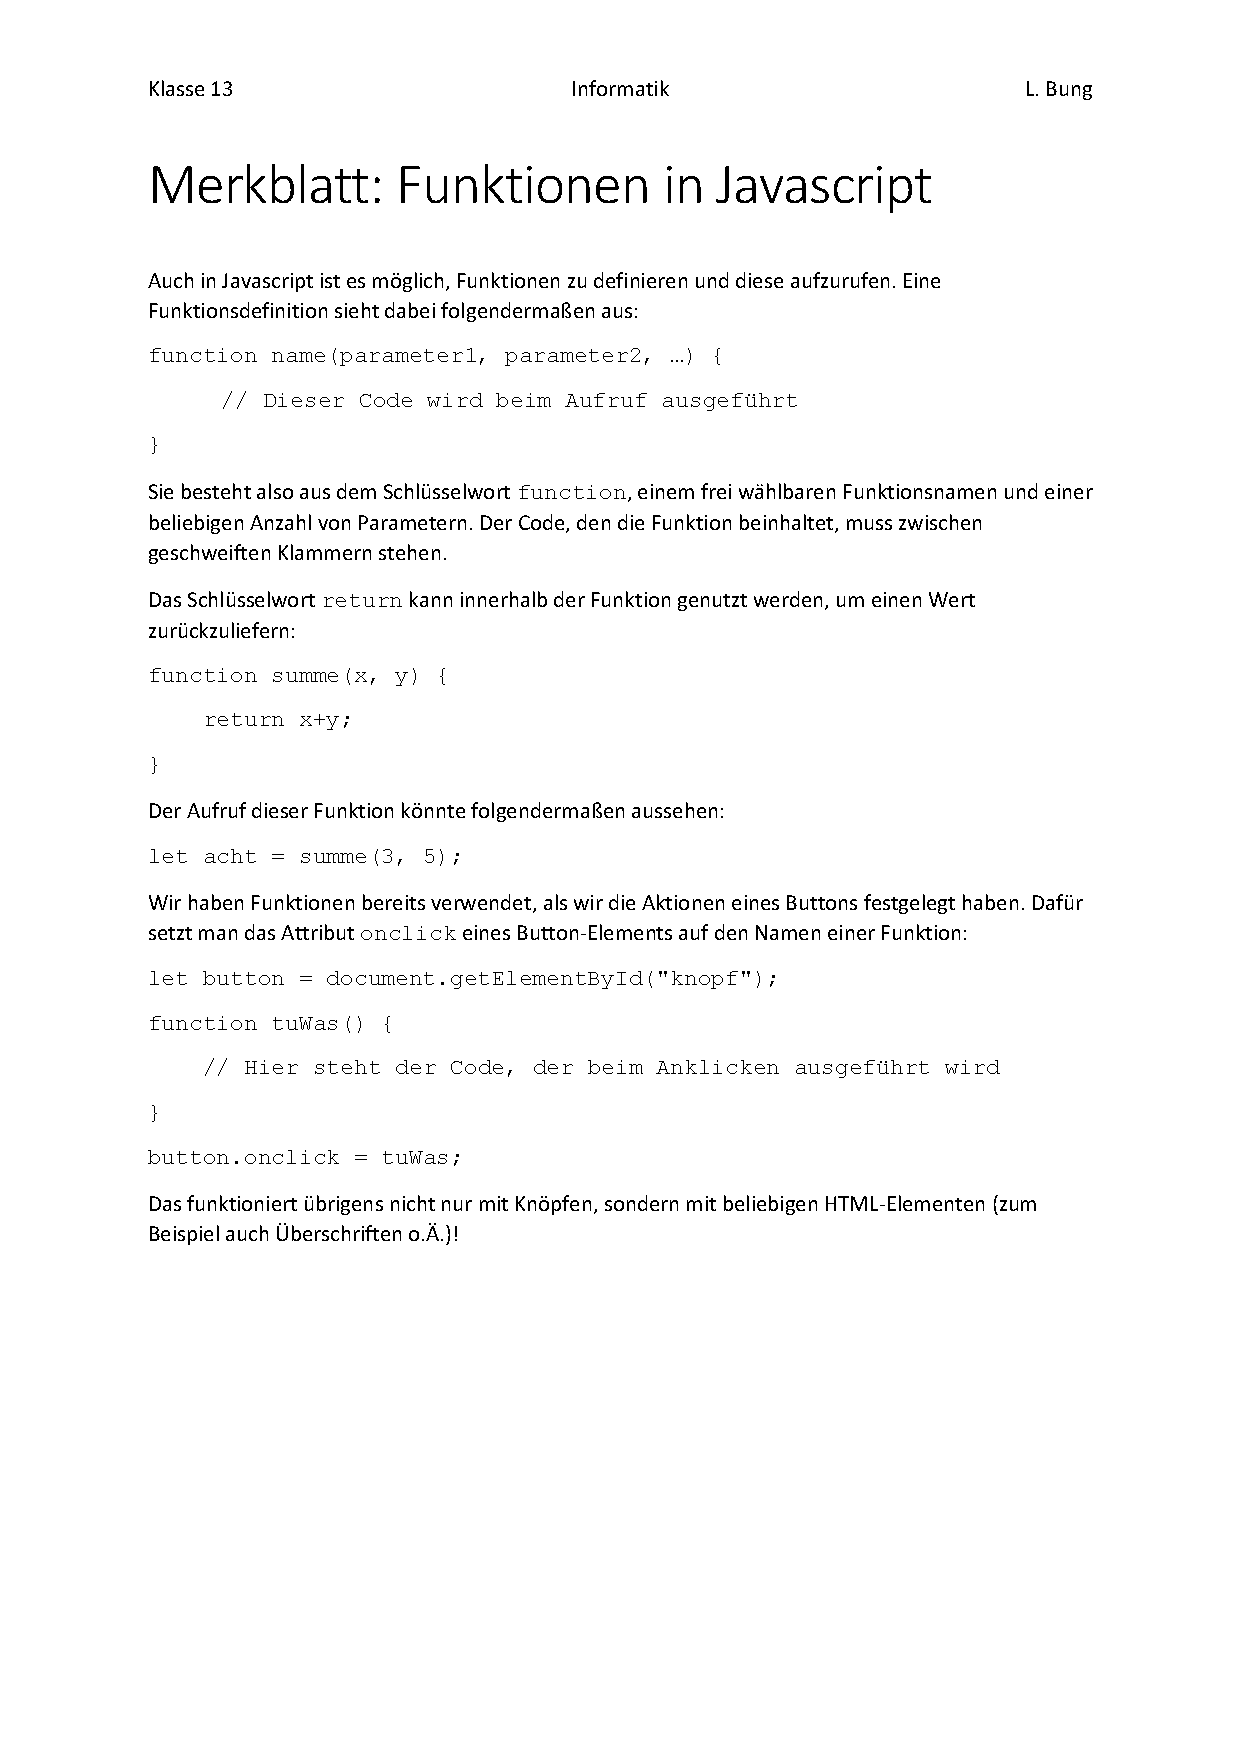
\includepdf[pages={-}, scale=0.8, frame, pagecommand={\thispagestyle{plain}},
addtotoc={1, subsection, 2, Merkblatt Funktionen, subsec:merkblatt_funktionen}]{appendix/Javascript4/Merkblatt_Funktionen.pdf}
\label{pdf:merkblatt_funktionen}


\section{Übungsblätter}
\label{app:übungsblätter}
\pagebreak

\phantomsection
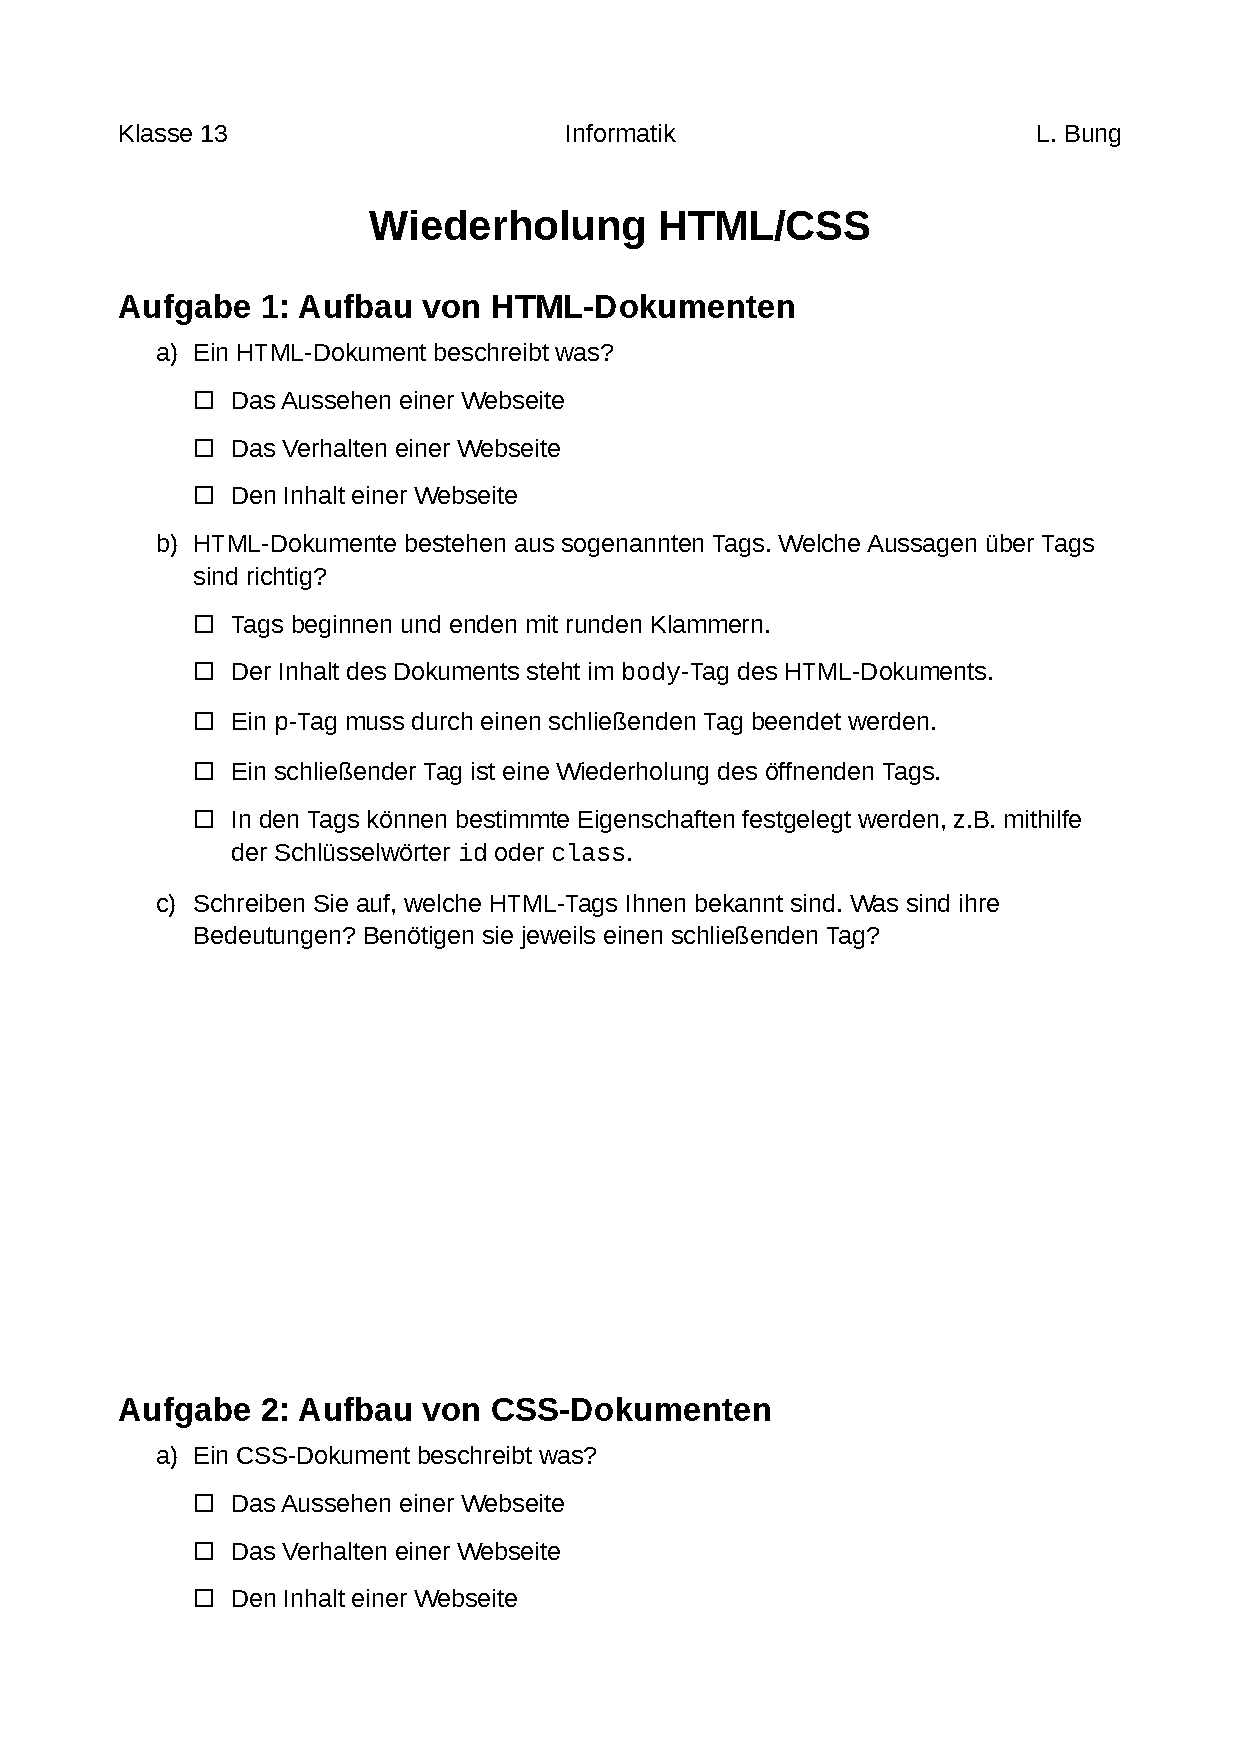
\includepdf[pages={-}, scale=0.8, frame, pagecommand={\thispagestyle{plain}},
addtotoc={1, subsection, 2, Übungsblatt HTML/CSS, subsec:ab_html_css}]{appendix/Javascript1/AB_HTML_CSS.pdf}
\label{pdf:ab_html_css}
\pagebreak

\phantomsection
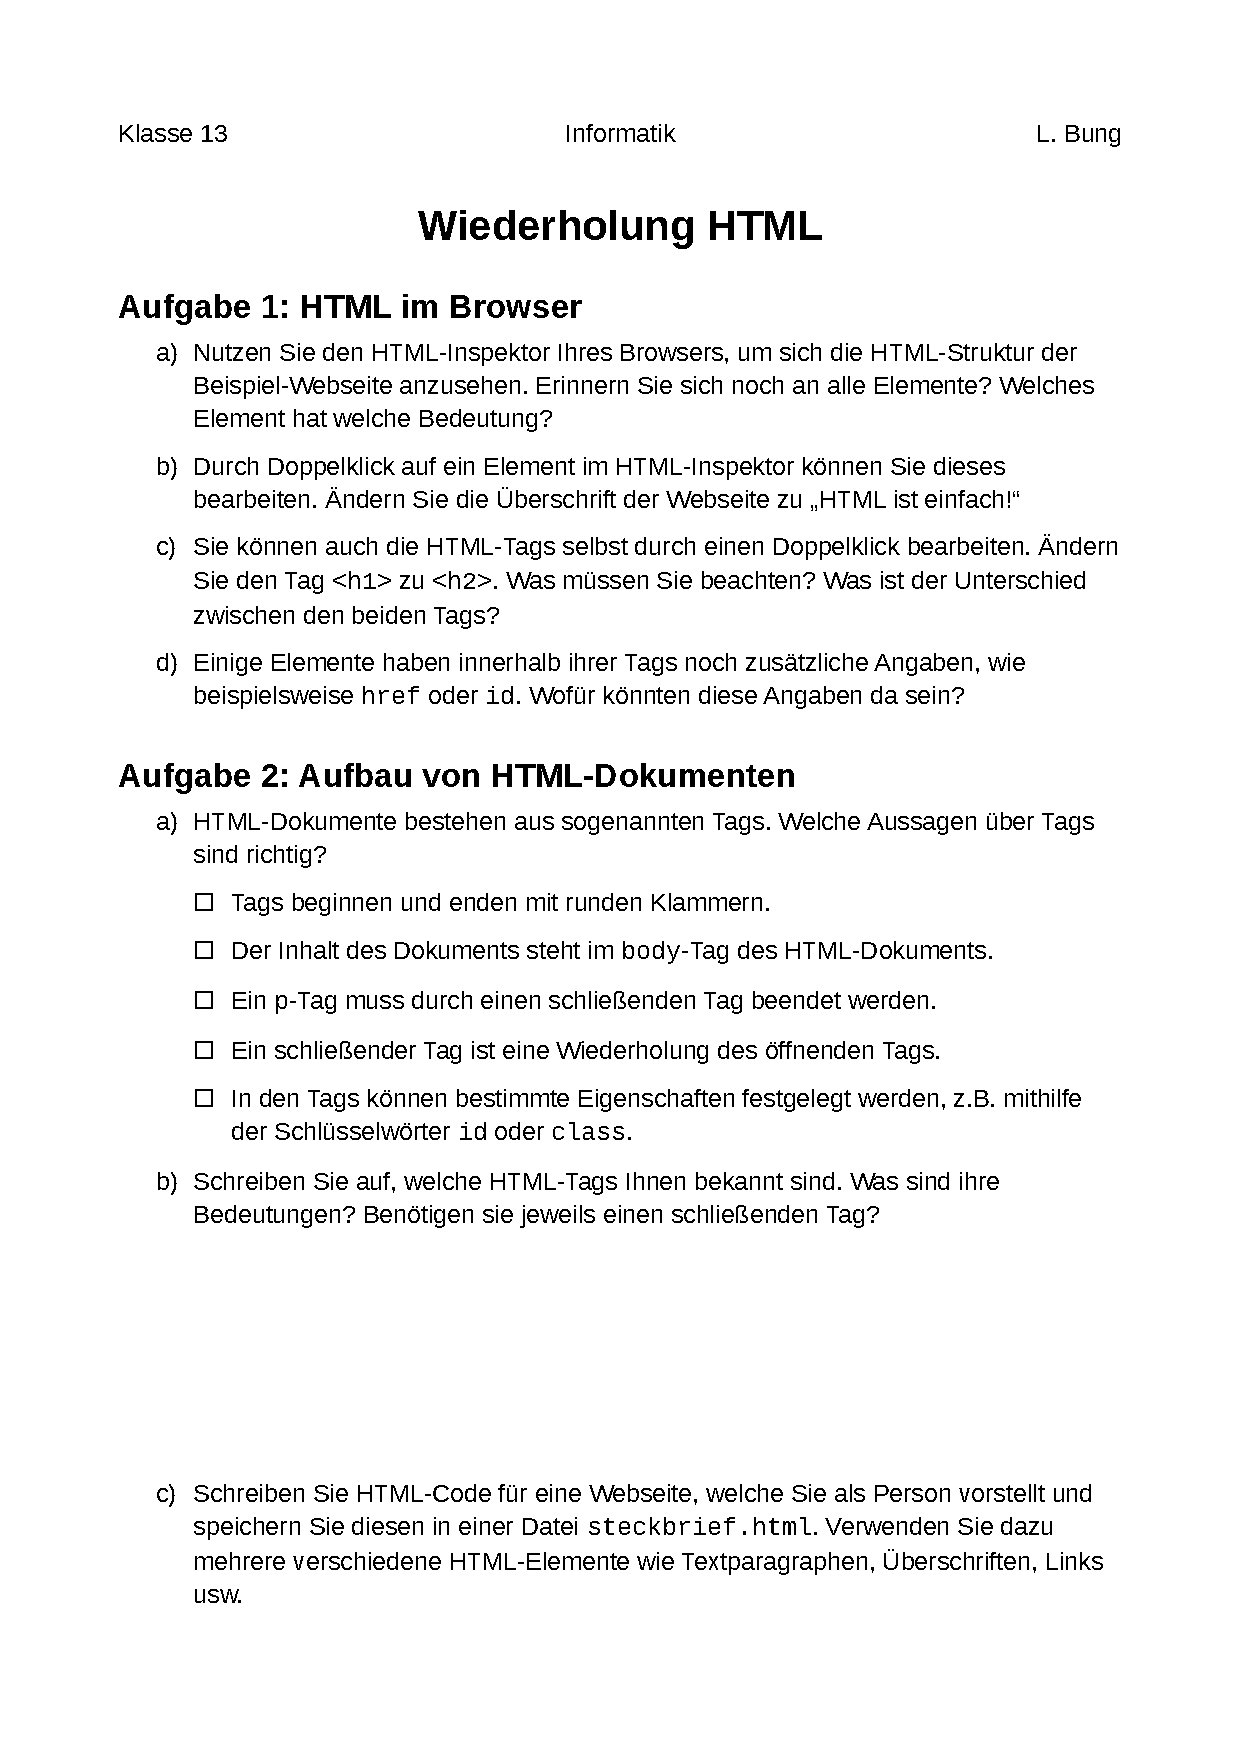
\includepdf[pages={-}, scale=0.8, frame, pagecommand={\thispagestyle{plain}},
addtotoc={1, subsection, 2, Übungsblatt HTML, subsec:ab_html}]{appendix/Javascript1/AB_HTML.pdf}
\label{pdf:ab_html}
\pagebreak

\phantomsection
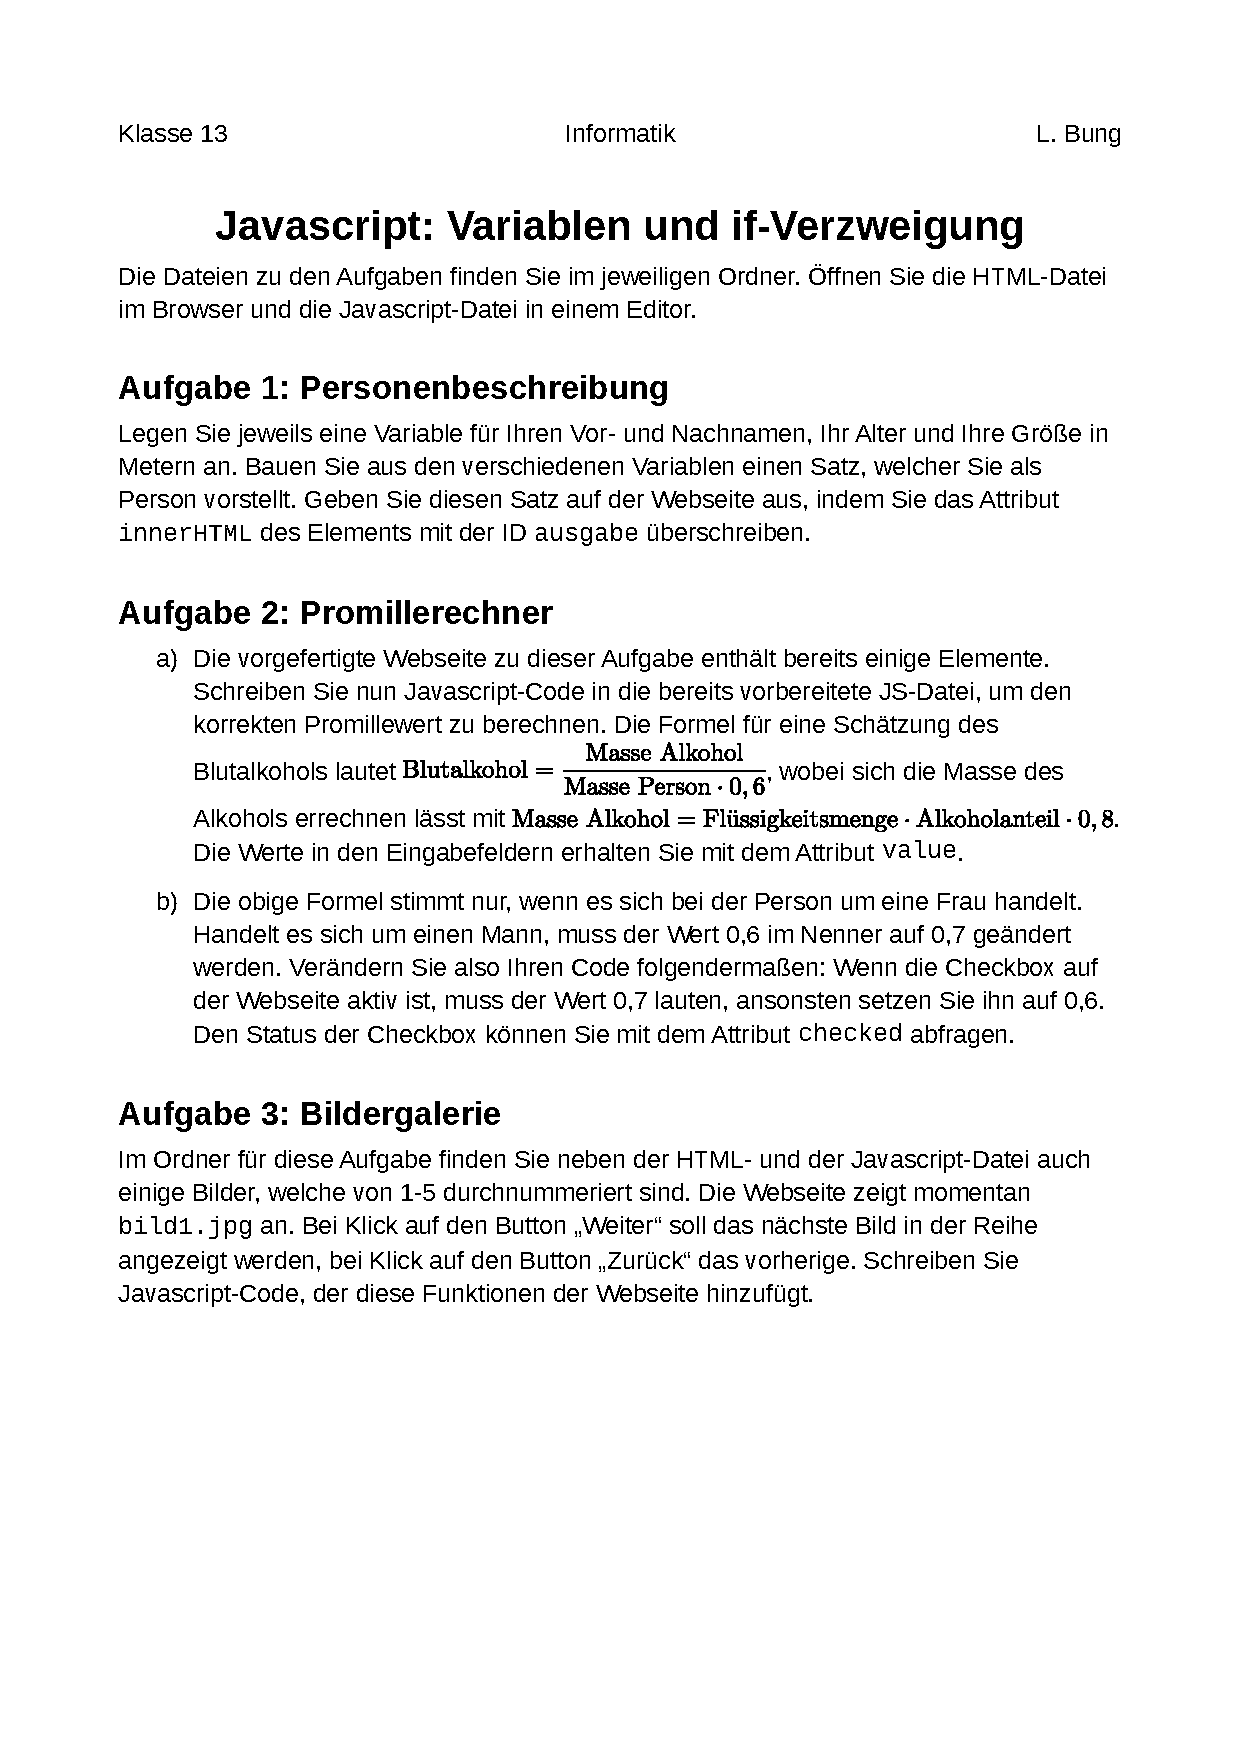
\includepdf[pages={-}, scale=0.8, frame, pagecommand={\thispagestyle{plain}},
addtotoc={1, subsection, 2, Übungsblatt Variablen/if, subsec:ab_variablen_if}]{appendix/Javascript1/AB_Variablen_if.pdf}
\label{pdf:ab_variablen_if}
\pagebreak

\phantomsection
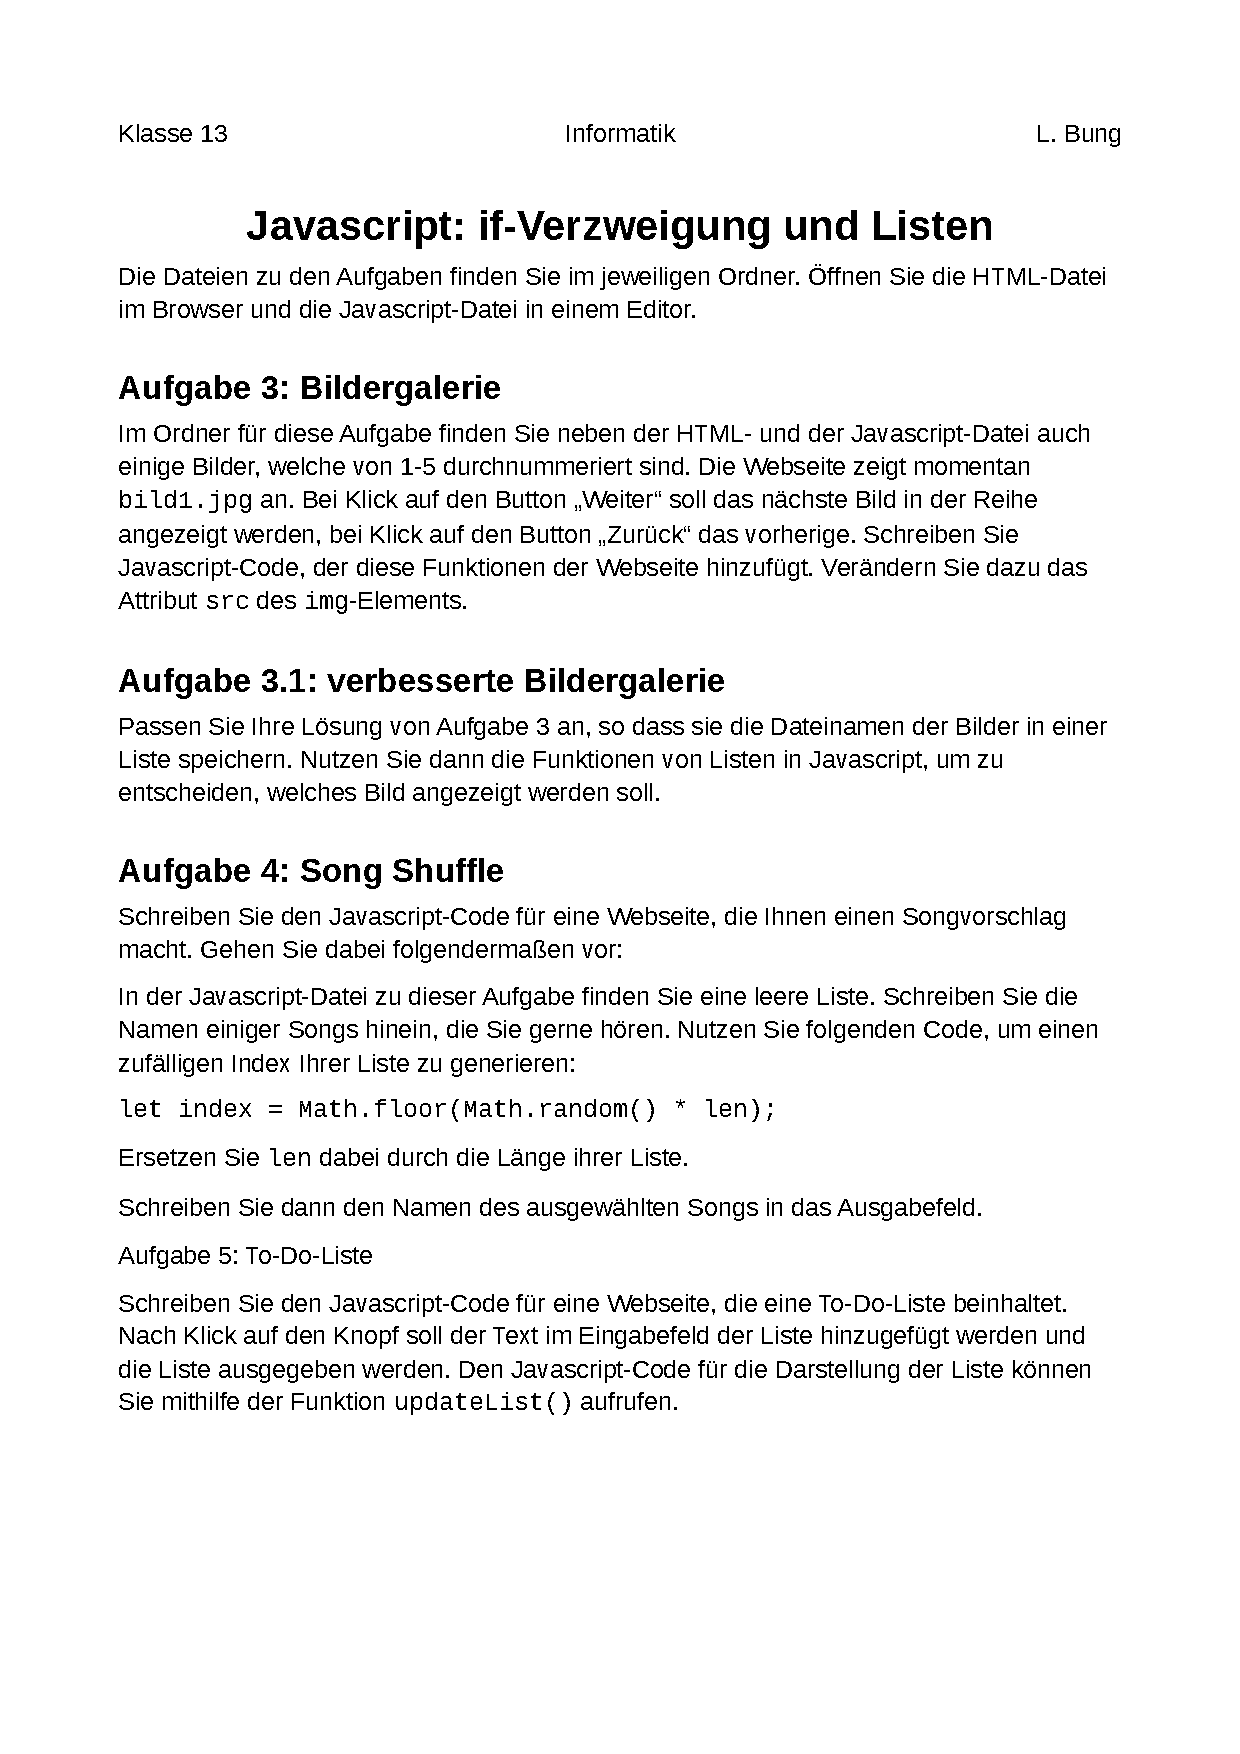
\includepdf[pages={-}, scale=0.8, frame,
pagecommand={\thispagestyle{plain}},
addtotoc={1, subsection, 2, Übungsblatt if/Listen, subsec:ab_if_listen}]{appendix/Javascript3/AB_if_Listen.pdf}
\label{pdf:ab_if_listen}
\pagebreak

\phantomsection

\includepdf[pages={-}, scale=0.8, frame,
pagecommand={\thispagestyle{plain}},
addtotoc={1, subsection, 2, Übungsblatt Funktionen, subsec:ab_funktionen}]{appendix/Javascript4/AB_Funktionen.pdf}
\label{pdf:ab_funktionen}

\section{Codegerüste zu den Übungsaufgaben}
\label{app:codegerüste}

\subsection{Aufgabe 0: Wiederholung HTML}
\label{app:code0}

\lstinputlisting[style=htmlcssjs, label=lst:code0, , caption={HTML-Code zu Aufgabe 0: Wiederholung HTML}]{appendix/Aufgaben/Aufgabe0/aufgabe0.html}


\subsection{Aufgabe 1: Personenbeschreibung}
\label{app:code1}

\lstinputlisting[style=htmlcssjs, label=lst:code1-html, caption={HTML-Code zu Aufgabe 1: Personenbeschreibung}]{appendix/Aufgaben/Aufgabe1/aufgabe1.html}

\lstinputlisting[style=htmlcssjs, label=lst:code1-js, caption={Javascript-Codegerüst zu Aufgabe 1: Personenbeschreibung}]{appendix/Aufgaben/Aufgabe1/aufgabe1.js}


\subsection{Aufgabe 2: Promillerechner}
\label{app:code2}

\lstinputlisting[style=htmlcssjs, label=lst:code2-html, caption={HTML-Code zu Aufgabe 2: Promillerechner}]{appendix/Aufgaben/Aufgabe2/aufgabe2.html}

\lstinputlisting[style=htmlcssjs, label=lst:code2-js, caption={Javascript-Codegerüst zu Aufgabe 2: Promillerechner}]{appendix/Aufgaben/Aufgabe2/aufgabe2.js}


\subsection{Aufgabe 3: Bildergalerie}
\label{app:code3}

\lstinputlisting[style=htmlcssjs, label=lst:code3-html, caption={HTML-Code zu Aufgabe 3: Bildergalerie}]{appendix/Aufgaben/Aufgabe3/aufgabe3.html}

\lstinputlisting[style=htmlcssjs, label=lst:code3-js, caption={Javascript-Codegerüst zu Aufgabe 3: Bildergalerie}]{appendix/Aufgaben/Aufgabe3/aufgabe3.js}


\subsection{Aufgabe 4: Song Shuffle}
\label{app:code4}

\lstinputlisting[style=htmlcssjs, label=lst:code4-html, caption={HTML-Code zu Aufgabe 4: Song Shuffle}]{appendix/Aufgaben/Aufgabe4/aufgabe4.html}

\lstinputlisting[style=htmlcssjs, label=lst:code4-js, caption={Javascript-Codegerüst zu Aufgabe 4: Song Shuffle}]{appendix/Aufgaben/Aufgabe4/aufgabe4.js}


\subsection{Aufgabe 5: To-Do-Liste}
\label{app:code5}

\lstinputlisting[style=htmlcssjs, label=lst:code5-html, caption={HTML-Code zu Aufgabe 5: To-Do-Liste}]{appendix/Aufgaben/Aufgabe5/aufgabe5.html}

\lstinputlisting[style=htmlcssjs, label=lst:code5-js, caption={Javascript-Codegerüst zu Aufgabe 5: To-Do-Liste}]{appendix/Aufgaben/Aufgabe5/aufgabe5.js}


\subsection{Aufgabe 6: Taschenrechner 1}
\label{app:code6}

\lstinputlisting[style=htmlcssjs, label=lst:code6-html, caption={HTML-Code zu Aufgabe 6: Taschenrechner 1}]{appendix/Aufgaben/Aufgabe6/aufgabe6.html}


\subsection{Aufgabe 7: Klickzähler}
\label{app:code7}

\lstinputlisting[style=htmlcssjs, label=lst:code7-html, caption={HTML-Code zu Aufgabe 7: Klickzähler}]{appendix/Aufgaben/Aufgabe7/aufgabe7.html}


\subsection{Aufgabe 8: Taschenrechner 2}
\label{app:code8}

\lstinputlisting[style=htmlcssjs, label=lst:code8-html, caption={HTML-Code zu Aufgabe 8: Taschenrechner 2}]{appendix/Aufgaben/Aufgabe8/aufgabe8.html}


\section{Ausdrucke der ersten Seiten der Onlineliteratur}
\pagebreak

\phantomsection

\includepdf[pages={1}, scale=0.7, frame,
pagecommand={\thispagestyle{plain} \cite{bildungsplan-tg-informatik}}]{onlinequellen/Bildungsplan_Beruflich_TG_Informatik.pdf}
\pagebreak

\phantomsection
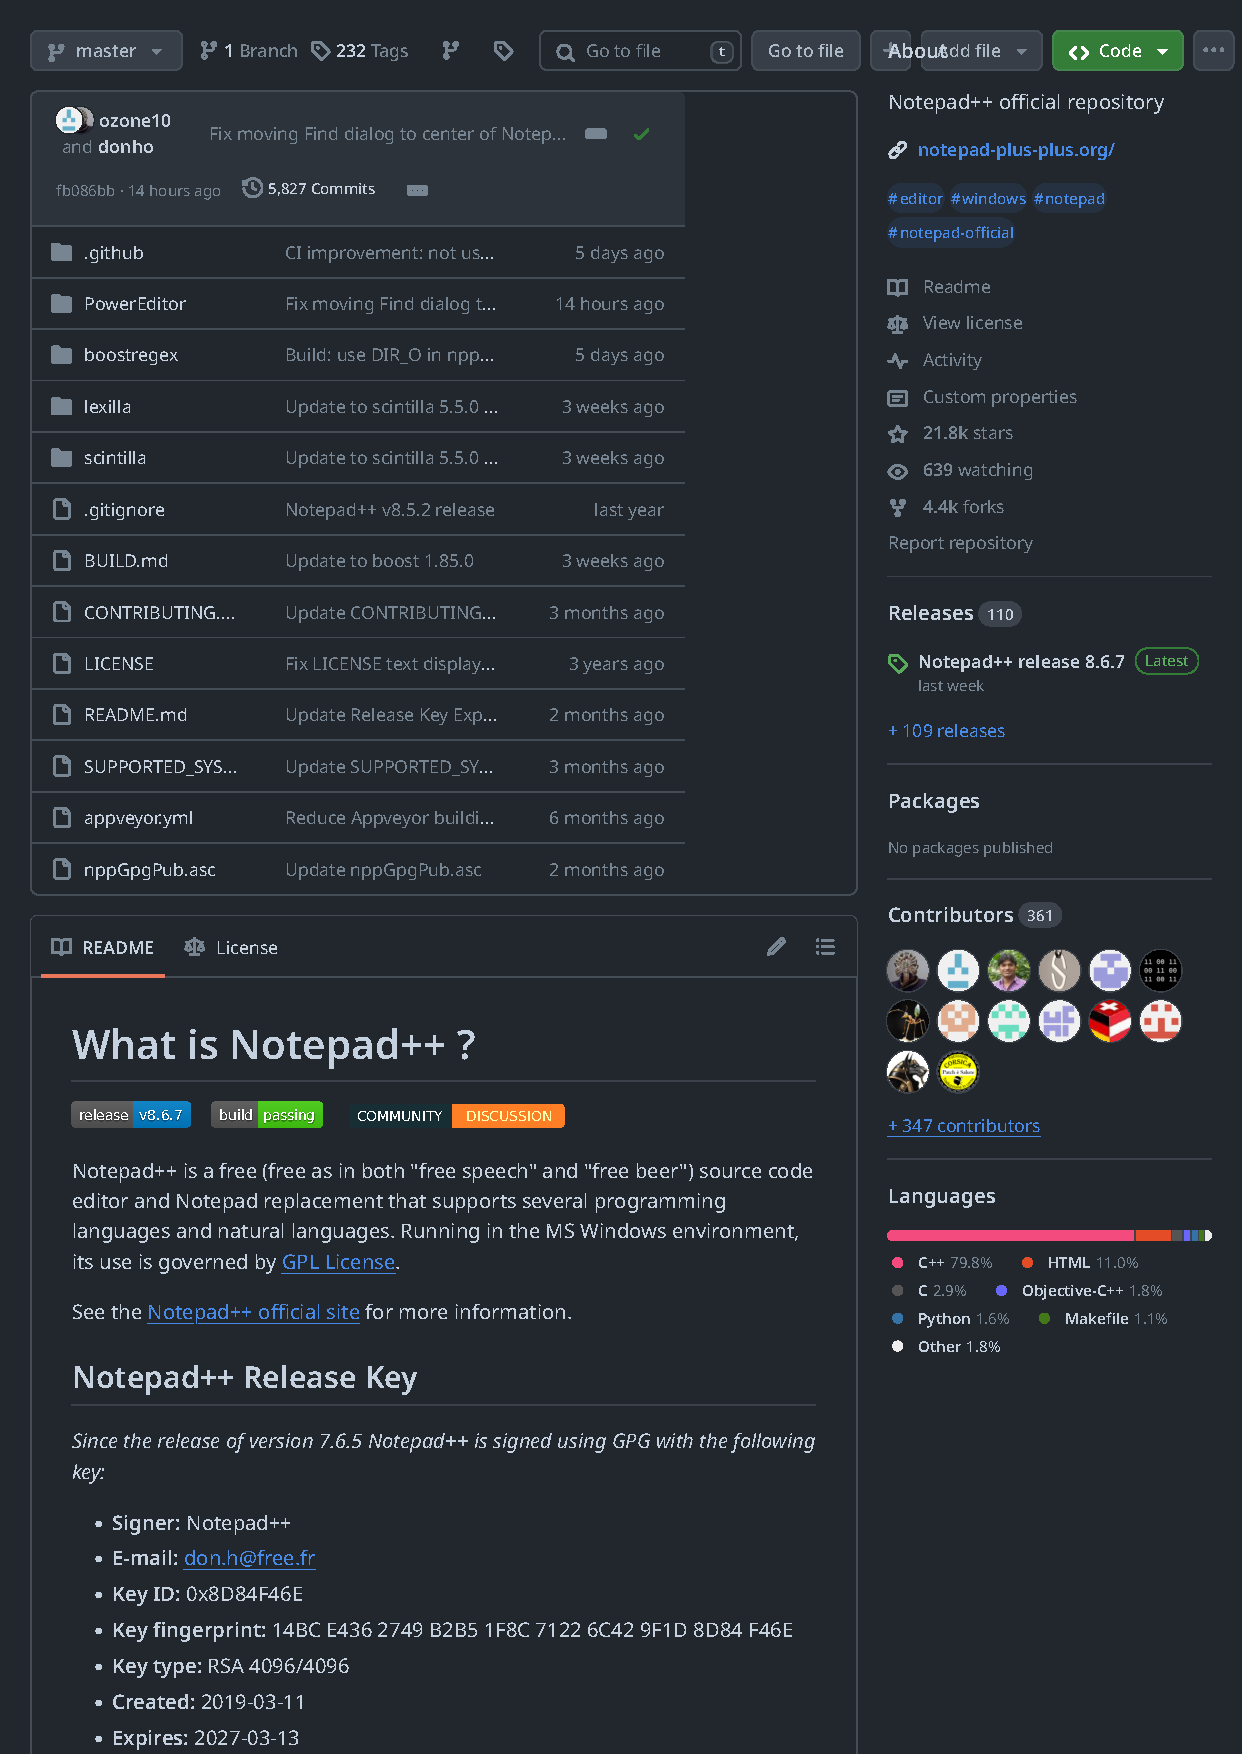
\includepdf[pages={1}, scale=0.7, frame,
pagecommand={\thispagestyle{plain} \cite{ho2021notepad++}}]{onlinequellen/notepad++_github.pdf}
\pagebreak

\phantomsection
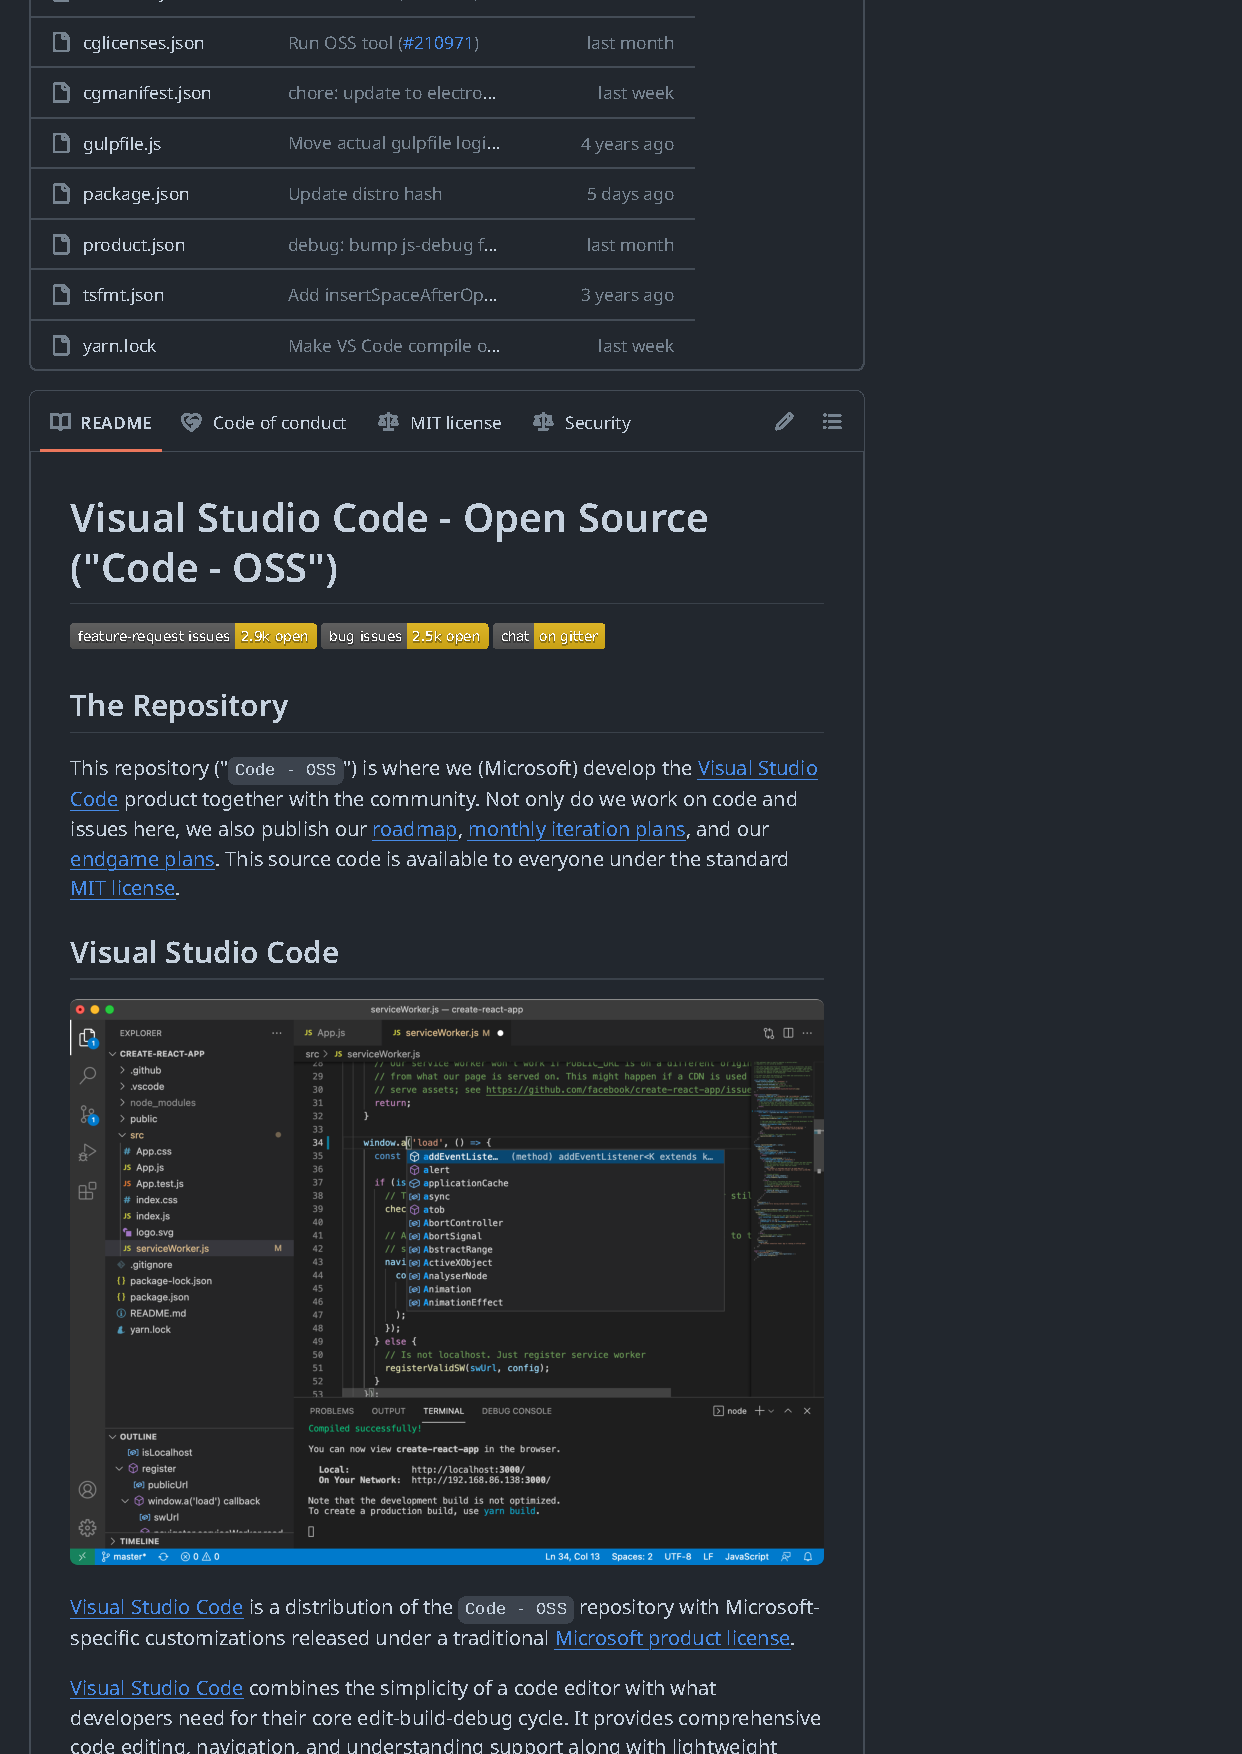
\includepdf[pages={1}, scale=0.7, frame,
pagecommand={\thispagestyle{plain} \cite{microsoft2024vscode}}]{onlinequellen/vscode_github.pdf}

\phantomsection

\includepdf[pages={1}, scale=0.7, frame,
pagecommand={\thispagestyle{plain}
\cite{handreichung-praxissemester}}]{onlinequellen/Handreichung_Praxissemester.pdf}
\end{appendices}
\end{document}